%%%%%%%%%%%%%%%%%%%%%%%%%%%%%%%%%%%%%%%%%%%%%%%%%%%%%%%%%%%%%%%%%%%%%%%%%%%%%%%%%%
 \begin{frame}[fragile]\frametitle{}
\begin{center}
{\Large Game Theory}

 -   Eric Rasmusen, Erasmuse@indiana.edu. http://www.rasmusen.org/
\end{center}
\end{frame}


%%%%%%%%%%%%%%%%%%%%%%%%%%%%%%%%%%%%%%%%%%%%%%%%%%%%%%%%%%%
 \begin{frame}[fragile]\frametitle{Definitions}

Game theory is concerned with the actions of decision makers who are conscious
that their actions affect each other.  When the only two publishers in a city
choose prices for their newspapers, aware that their sales are determined
jointly, they are players in a game with each other. They are not in a game with
the readers who buy the newspapers, because each reader ignores his   effect on
the publisher. Game theory is not useful when decisionmakers ignore the
reactions of others or treat them as impersonal market forces.

\end{frame}

%%%%%%%%%%%%%%%%%%%%%%%%%%%%%%%%%%%%%%%%%%%%%%%%%%%%%%%%%%%
 \begin{frame}[fragile]\frametitle{Definitions}
 The best way to understand which situations can be modelled as games and which
cannot is to think about examples like  the following:
\begin{enumerate}
 \item
OPEC members choosing their annual output;

\item General Motors purchasing steel from USX;

\item two manufacturers, one of nuts and one of bolts, deciding whether to use
metric or American standards;

\item a board of directors setting up a stock option plan for the chief
executive officer;

\item the US Air Force hiring  jet fighter pilots;

\item an electric company deciding whether to order a new power plant given its
estimate of demand for electricity in ten years. \end{enumerate}
\end{frame}


%%%%%%%%%%%%%%%%%%%%%%%%%%%%%%%%%%%%%%%%%%%%%%%%%%%%%%%%%%%
 \begin{frame}[fragile]\frametitle{Definitions}
The first four examples are games.  In (1), OPEC members are playing a
game because Saudi Arabia knows that Kuwait's oil output is based on Kuwait's
forecast of Saudi output, and the output from both countries matters to the
world price. In  (2), a significant portion of American trade in steel is
between General Motors and USX, companies which realize that the quantities
traded by each of them affect the price. One wants the price low, the other
high, so this is a game with conflict between the two players.  In  (3), the nut
and bolt manufacturers are not in conflict, but the actions of one  do affect
the desired actions of the other, so the situation is a game none the less. In
(4),  the board of directors chooses a stock option plan anticipating the effect
on the actions of the CEO.
\end{frame}

%%%%%%%%%%%%%%%%%%%%%%%%%%%%%%%%%%%%%%%%%%%%%%%%%%%%%%%%%%%
 \begin{frame}[fragile]\frametitle{Definitions}
 Game theory is inappropriate for modelling the final two examples. In (5),
each individual  pilot affects the US Air Force insignificantly, and each pilot
makes his employment decision without regard for the impact on the Air Force's
policies.     In (6), the electric company faces a complicated decision, but it
does not face another rational agent. These situations are more appropriate for
the use of {\bf decision theory} than game theory, decision theory being the
careful analysis of how one person makes a decision when he may be faced with
uncertainty, or an entire sequence of decisions that interact with each other,
but when he is not faced with having to interact strategically with other single
decision makers. Changes in the important economic variables could,however,
turn examples (5) and (6) into games. The appropriate model changes if  the Air
Force faces a pilots' union or if the public utility commission pressures the
utility to change its generating capacity.

\end{frame}


%%%%%%%%%%%%%%%%%%%%%%%%%%%%%%%%%%%%%%%%%%%%%%%%%%%%%%%%%%%
 \begin{frame}[fragile]\frametitle{Definitions}
  Game theory as it will be presented in this book is a modelling tool, not an
axiomatic system.  The presentation in this chapter is unconventional. Rather
than starting with mathematical definitions or simple little games of the kind
used later in the chapter, we will start with a situation to be modelled, and
build a game from it step by step.

\end{frame}

%%%%%%%%%%%%%%%%%%%%%%%%%%%%%%%%%%%%%%%%%%%%%%%%%%%%%%%%%%%
 \begin{frame}[fragile]\frametitle{Describing a Game}
The essential elements of a game are {\bf players}, {\bf actions},
{\bf payoffs}, and {\bf information}-- PAPI, for short.   These are collectively
known as the {\bf rules of the game}, and the modeller's objective is to
describe a situation  in terms of the rules of a game so as to explain what
will happen in that situation.  Trying to maximize their payoffs, the players
will devise plans known as {\bf strategies} that pick actions depending on the
information that has arrived at each moment. The combination of strategies
chosen by each player is known as the {\bf equilibrium}. Given an equilibrium,
the modeller can see what actions come out of the conjunction of all the
players'  plans, and this tells him the {\bf outcome} of the game.

\end{frame}

%%%%%%%%%%%%%%%%%%%%%%%%%%%%%%%%%%%%%%%%%%%%%%%%%%%%%%%%%%%
 \begin{frame}[fragile]\frametitle{Describing a Game}
  This kind of  standard  description helps both the modeller and his readers.
For the modeller, the names are useful because they help ensure that the
important details of the game have been fully specified. For his readers, they
make the game easier to understand, especially if, as with most technical
papers, the paper is first skimmed quickly to see if it is worth reading. The
less clear a writer's style, the more closely he should adhere to the standard
names, which means that most of us ought to adhere very closely indeed.
\end{frame}


%%%%%%%%%%%%%%%%%%%%%%%%%%%%%%%%%%%%%%%%%%%%%%%%%%%%%%%%%%%
 \begin{frame}[fragile]\frametitle{Describing a Game}
  Think of writing a paper as a game between author and reader, rather than as a
single-player production process.  The author, knowing that he has valuable
information but imperfect means of communication, is trying to convey the
information to the reader. The reader does not know whether the information is
valuable, and he must choose whether to read the paper closely enough to find
out.\footnote{Once you have read to the end of this chapter:  What are the
possible equilibria of this game?}
\end{frame}



%%%%%%%%%%%%%%%%%%%%%%%%%%%%%%%%%%%%%%%%%%%%%%%%%%%%%%%%%%%
 \begin{frame}[fragile]\frametitle{Describing a Game}
To define the  terms used above  and to show the difference between game theory
and decision theory,  let us use the example of an entrepreneur trying to decide
whether to start a dry cleaning store in a   town   already served by one dry
cleaner.  We will call the two firms ``NewCleaner'' and ``OldCleaner.''
NewCleaner  is uncertain about whether the economy will be in a recession or
not,  which will affect how much consumers pay for dry cleaning,   and must also
worry about whether OldCleaner will respond to entry with a price war or by
keeping its initial high prices.  OldCleaner is a well-established firm, and it
would survive any price war, though its profits would fall. NewCleaner must
itself decide whether to initiate a price war or to charge high prices, and must
also decide what kind of equipment to buy, how many workers to hire, and so
forth.
\end{frame}


%%%%%%%%%%%%%%%%%%%%%%%%%%%%%%%%%%%%%%%%%%%%%%%%%%%%%%%%%%%
 \begin{frame}[fragile]\frametitle{Describing a Game}
{\it{\bf Players} are the individuals who make decisions. Each
player's goal is to maximize his utility by choice of actions.}

In the Dry Cleaners Game,   let us specify the players to be NewCleaner and
OldCleaner. Passive individuals like the customers, who react predictably to
price changes without any thought of trying to change anyone's behavior, are not
players, but environmental parameters. Simplicity is the goal in modelling, and
the ideal is to keep the number of players down to the minimum that captures the
essence of the situation.
\end{frame}


%%%%%%%%%%%%%%%%%%%%%%%%%%%%%%%%%%%%%%%%%%%%%%%%%%%%%%%%%%%
 \begin{frame}[fragile]\frametitle{Describing a Game}

Sometimes   it is  useful to explicitly include individuals in the model called
{\bf pseudo-players} whose actions are taken in a purely mechanical way.

 {\it {\bf Nature} is a pseudo-player who takes random actions at
specified points in the game with specified probabilities.}

  In the Dry Cleaners Game, we will model  the possibility of recession as a
move by Nature.  With probability 0.3, Nature decides that there will be a
recession, and with probability 0.7 there will not.       Even if the players
always took the same actions, this random move means that the model would yield
more than just one prediction. We say that there are different {\bf
realizations} of a game depending on the results of random moves.
\end{frame}


%%%%%%%%%%%%%%%%%%%%%%%%%%%%%%%%%%%%%%%%%%%%%%%%%%%%%%%%%%%
 \begin{frame}[fragile]\frametitle{Describing a Game}

 {\it An {\bf action} or {\bf move} by player $i$, denoted $a_{i},$ is
a choice he can make.}

 {\it Player $i$'s {\bf action set}, $A_i = \{a_{i}\}$, is the entire
set of actions available to him.}

 {\it An {\bf action combination} is a list $a =\{a_i\},\; (i=
1,\ldots,n)$ of one action for each of the $n$ players in the game.}
\end{frame}

%%%%%%%%%%%%%%%%%%%%%%%%%%%%%%%%%%%%%%%%%%%%%%%%%%%%%%%%%%%
 \begin{frame}[fragile]\frametitle{Describing a Game}

 Again, simplicity is our goal.  We are trying to determine whether Newcleaner
will enter or not, and for this  it is not important for us to go into the
technicalities of dry cleaning equipment and labor practices.   Also, it will
not be in Newcleaner's  interest to start a price war, since it cannot possibly
drive out Oldcleaners, so we can exclude that decision from our model.
Newcleaner's action set can be modelled very simply as  $  \{ Enter, Stay \;
Out\}$.  We will also specify  Oldcleaner's action set to be  simple: it is to
choose price from   $  \{ Low,   High\}$.
\end{frame}



%%%%%%%%%%%%%%%%%%%%%%%%%%%%%%%%%%%%%%%%%%%%%%%%%%%%%%%%%%%
 \begin{frame}[fragile]\frametitle{Describing a Game}

{\it By player $i$'s {\bf payoff} $\pi_i(s_1,\ldots,s_n)$, we mean
either:\\ (1) The utility player $i$ receives after all players and Nature have
picked their strategies and the game has been played out; or\\ (2) The expected
utility he receives as a function of the strategies chosen by himself and the
other players.}
\end{frame}

%%%%%%%%%%%%%%%%%%%%%%%%%%%%%%%%%%%%%%%%%%%%%%%%%%%%%%%%%%%
 \begin{frame}[fragile]\frametitle{Describing a Game}


   For the moment, think of ``strategy'' as a synonym for ``action''.
Definitions (1) and (2) are distinct and different, but in the literature and
this book the term ``payoff'' is used for both the actual payoff and the
expected payoff. The context will make clear which is meant.  If one is
modelling  a particular  real-world situation,  figuring out the payoffs is
often the hardest part of constructing a model.  For this pair of dry cleaners,
we will pretend we have looked over all the data and figured out that the
payoffs are as given by Table  1a   if the economy is normal, and that if there
is a recession   the  payoff of each player who   operates in the market is
60 thousand dollars lower, as shown in Table next.
\end{frame}

%%%%%%%%%%%%%%%%%%%%%%%%%%%%%%%%%%%%%%%%%%%%%%%%%%%%%%%%%%%
 \begin{frame}[fragile]\frametitle{Describing a Game}
 \begin{center} {\bf Table 1a:  The Dry Cleaners Game: Normal Economy}

 \begin{tabular}{lllccc} &       &             &\multicolumn{3}{c}{\bf
OldCleaner}\\ &       &             &   {\it Low price}  &   & {\it High price}
\\ &   &  {\it Enter}      &     -100, -50 &    &100, 100 \\ & {\bf NewCleaner}
&& & &   \\ &  &       {\it   Stay Out}     &      0,50   &    &  0,300  \\
\multicolumn{6}{l}{ Payoffs to: (NewCleaner, OldCleaner) in thousands of dollars
} \end{tabular} \end{center}

  \begin{center} {\bf Table 1b:  The Dry Cleaners Game: Recession}

 \begin{tabular}{lllccc} &       &             &\multicolumn{3}{c}{\bf
OldCleaner}\\ &       &             &   {\it Low price}  &   & {\it High price}
\\ &   &  {\it Enter}      &     -160, -110 &    &40, 40 \\ & {\bf NewCleaner}
&& & &   \\ &  &       {\it   Stay Out}     &      0,-10   &    &  0,240  \\
\multicolumn{6}{l}{ Payoffs to: (NewCleaner, OldCleaner) in thousands of dollars
} \end{tabular} \end{center}
\end{frame}

%%%%%%%%%%%%%%%%%%%%%%%%%%%%%%%%%%%%%%%%%%%%%%%%%%%%%%%%%%%
 \begin{frame}[fragile]\frametitle{Describing a Game}
  Information is modelled using the concept of the {\bf information set}, a
concept which will be defined more precisely in Section 2.2. For now, think of a
player's information set as his knowledge at a particular time of the values of
different variables. The elements of the information set are the different
values that the player thinks are possible. If the information set has many
elements, there are many values the player cannot rule out; if it has one
element, he knows the value precisely.  A player's information set includes not
only distinctions between the values of variables such as the strength of oil
demand, but also knowledge of what actions have previously been taken, so his
information set changes over the course of the game.
\end{frame}

%%%%%%%%%%%%%%%%%%%%%%%%%%%%%%%%%%%%%%%%%%%%%%%%%%%%%%%%%%%
 \begin{frame}[fragile]\frametitle{Describing a Game}
  Here,  at the time that it chooses its price,  OldCleaner will know
NewCleaner's decision about entry.  But what do the firms know about the
recession?  If both firms know about the recession we model that as Nature
moving before NewCleaner; if  only OldCleaner knows, we put Nature's move after
NewCleaner; if neither firm knows whether there is a recession at the time they
must make their decisions, we put Nature's move at the end of the game.  Let us
do this last.
\end{frame}



%%%%%%%%%%%%%%%%%%%%%%%%%%%%%%%%%%%%%%%%%%%%%%%%%%%%%%%%%%%
 \begin{frame}[fragile]\frametitle{Describing a Game}
       It is convenient to lay out information and actions together in an {\bf
order of play}.  Here is the  order of play we have specified for the Dry
Cleaners Game:

  1   Newcleaner chooses its entry decision from $  \{ Enter,  Stay \;
Out\}$.\\  2  Oldcleaner chooses its  price   from $  \{ Low,   High\}
$.  \\  3  Nature picks demand, $D$, to be $Recession$ with probability
0.3 or $Normal$ with probability 0.7.\\
\end{frame}

%%%%%%%%%%%%%%%%%%%%%%%%%%%%%%%%%%%%%%%%%%%%%%%%%%%%%%%%%%%
 \begin{frame}[fragile]\frametitle{Describing a Game}
   The purpose of modelling is to explain how  a given set of circumstances
leads to a particular result. The  result of interest is known as the outcome.

 {\it The {\bf outcome} of the game is a set of interesting elements
that the modeller picks from the values of actions, payoffs, and other variables
after the game is played out.}

   The definition of the outcome for any particular model depends on what
variables   the modeller finds interesting. One way to define the outcome of the
Dry Cleaners Game would be as either $Enter$ or {\it Stay Out}.  Another way,
appropriate if the model is being constructed to help plan  NewCleaner's
finances, is as the payoff that NewCleaner realizes, which is, from Tables 1a
and 1b,  one element of the set {\it \{0, 100, -100,  40, -160\}}.
\end{frame}

%%%%%%%%%%%%%%%%%%%%%%%%%%%%%%%%%%%%%%%%%%%%%%%%%%%%%%%%%%%
 \begin{frame}[fragile]\frametitle{Describing a Game}
  Having laid out the assumptions of the model, let us return to  what is
special about the way game theory models a situation. Decision theory  sets up
the rules of the game in  much the same way as game theory, but its outlook is
fundamentally different in one important way: there is only one player.   Return
to NewCleaner's decision about entry.   In decision theory,    the  standard
method is to  construct a {\bf decision tree} from the rules of the game, which
is just a graphical way to depict the order of play.

\end{frame}

%%%%%%%%%%%%%%%%%%%%%%%%%%%%%%%%%%%%%%%%%%%%%%%%%%%%%%%%%%%
 \begin{frame}[fragile]\frametitle{Describing a Game}
Figure 1 shows a decision tree for  the Dry Cleaners Game.   It shows all the
moves available to NewCleaner,  the probabilities of states of nature ( actions
that NewCleaner cannot control),  and the payoffs  to NewCleaner depending on
its choices and what the environment is like. Note that although we already
specified the probabilities of Nature's move to be 0.7 for $Normal$, we also
need to specify a probability for OldCleaner's move, which is set at probability
0.5 of {\it Low price} and probability 0.5 of {\it High price}.



 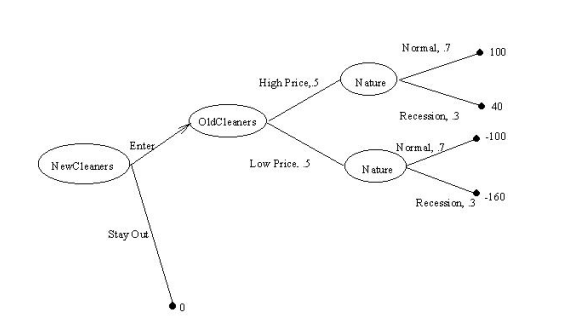
\includegraphics[width=0.5\linewidth,keepaspectratio]{fig01-01}



\begin{center} {\bf Figure 1:   The Dry Cleaners Game as a Decision Tree   }
\end{center}
\end{frame}

%%%%%%%%%%%%%%%%%%%%%%%%%%%%%%%%%%%%%%%%%%%%%%%%%%%%%%%%%%%
 \begin{frame}[fragile]\frametitle{Describing a Game}
Once a decision tree is set up, we can solve for the optimal decision which
maximizes the expected payoff.   Suppose NewCleaner has entered.  If  OldCleaner
chooses a high price, then  NewCleaner's expected payoff is 82, which is
0.7(100) + 0.3(40).  If  OldCleaner chooses a  low  price, then  NewCleaner's
expected payoff is  -118, which is 0.7(-100) + 0.3(-160). Since there is a 50-50
chance of each move by OldCleaner, NewCleaner's overall expected payoff from
{\it Enter} is  -18. That is worse than the 0 which NewCleaner could get by
choosing {\it stay out}, so the prediction is that NewCleaner will stay out.


\end{frame}

%%%%%%%%%%%%%%%%%%%%%%%%%%%%%%%%%%%%%%%%%%%%%%%%%%%%%%%%%%%
 \begin{frame}[fragile]\frametitle{Describing a Game}
That, however, is wrong.  This is a game, not  just a decision problem.  The
flaw in the reasoning I just went through is the assumption that OldCleaner will
choose {\it High price} with probability 0.5. If we use information about
OldCleaner' payoffs and figure out what moves OldCleaner will take  in solving
its own profit maximization problem, we will come to a different conclusion.


\end{frame}

%%%%%%%%%%%%%%%%%%%%%%%%%%%%%%%%%%%%%%%%%%%%%%%%%%%%%%%%%%%
 \begin{frame}[fragile]\frametitle{Describing a Game}
First, let us depict the order of play as a {\bf game tree} instead of  a
decision tree.  Figure  2 shows our model as a game tree, with all of
OldCleaner's moves and payoffs.




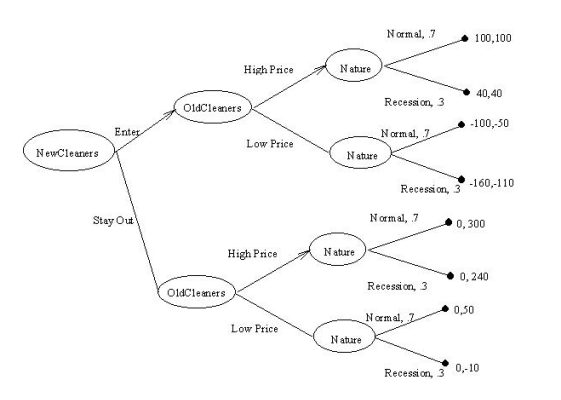
\includegraphics[width=0.5\linewidth,keepaspectratio]{fig01-02}

\begin{center} {\bf Figure  2:   The Dry Cleaners Game as a Game  Tree }
\end{center}


\end{frame}

%%%%%%%%%%%%%%%%%%%%%%%%%%%%%%%%%%%%%%%%%%%%%%%%%%%%%%%%%%%
 \begin{frame}[fragile]\frametitle{Describing a Game}
Viewing the situation as a game, we must think about both players' decision
making.  Suppose NewCleaner has entered. If OldCleaner chooses {\it High price},
OldCleaner's expected profit is  82, which is 0.7(100) + 0.3(40).   If
OldCleaner  chooses {\it  Low  price}, OldCleaner's expected profit is   -68,
which is 0.7(-50) + 0.3(-110). Thus, OldCleaner will choose  {\it High price},
and with probability 1.0, not 0.5. The arrow on the game tree for {\it High
price} shows this conclusion of our reasoning.  This means, in turn,  that
NewCleaner can predict an expected payoff of   82, which is 0.7(100) + 0.3(40),
from {\it Enter}.

\end{frame}

%%%%%%%%%%%%%%%%%%%%%%%%%%%%%%%%%%%%%%%%%%%%%%%%%%%%%%%%%%%
 \begin{frame}[fragile]\frametitle{Describing a Game}
  Suppose NewCleaner has not entered. If OldCleaner  chooses {\it High price},
OldCleaner' expected profit is  282, which is 0.7(300) + 0.3(240).   If
OldCleaner  chooses {\it  Low  price}, OldCleaner's expected profit is   32,
which is 0.7(50) + 0.3(-10).  Thus, OldCleaner will choose  {\it High price}, as
shown by the arrow on   {\it High price}.     If NewCleaner chooses {\it Stay
out}, NewCleaner will have a payoff of 0, and since that is worse than the 82
which NewCleaner can predict from {\it Enter}, NewCleaner will in fact enter the
market.

This switching back from the point of view of one player to the point of view of
another is characteristic of game theory.  The game theorist must practice
putting himself in {\it everybody} else's shoes.  (Does that mean we become
kinder, gentler people? -- Or do we just get trickier?)
\end{frame}


%%%%%%%%%%%%%%%%%%%%%%%%%%%%%%%%%%%%%%%%%%%%%%%%%%%%%%%%%%%
 \begin{frame}[fragile]\frametitle{Describing a Game}
Since so much depends on the interaction between the plans and predictions of
different players, it is useful to go a step beyond simply setting out actions
in a game.  Instead, the modeller goes on to think about {\bf strategies}, which
are action plans.

  {\it Player $i$'s {\bf strategy} $s_i$ is a rule that tells him which
action to choose at each instant of the game, given his information set.}

  {\it Player $i$'s {\bf strategy set} or {\bf strategy space} $S_i =
\{ s_i\}$ is the set of strategies available to him. }

  {\it A {\bf strategy profile} $s=(s_1,\ldots,s_n)$ is a list
consisting of one strategy for each of the {\rm n} players in the game.}
\footnote{ I used ``strategy combination'' instead of    ``strategy profile''
in the   third edition, but ``profile'' seems well enough established that I'm
switching to it.  }
\end{frame}


%%%%%%%%%%%%%%%%%%%%%%%%%%%%%%%%%%%%%%%%%%%%%%%%%%%%%%%%%%%
 \begin{frame}[fragile]\frametitle{Describing a Game}
Since the information set includes whatever the player knows about the previous
actions of other players, the strategy tells him how to react to their actions.
In The  Dry Cleaners Game,  the  strategy set for NewCleaner is just {\it \{
Enter, Stay Out \} }, since NewCleaner moves first and is not reacting to any
new information.  The strategy set for  OldCleaner, though, is

 \begin{center} $$ \left\{ \begin{tabular}{l} High Price if NewCleaner Entered,
Low Price if NewCleaner Stayed Out\\ Low Price if NewCleaner Entered,  High
Price if NewCleaner Stayed Out\\ High Price No Matter What\\ Low Price No Matter
What\\ \end{tabular} \right\} $$ \end{center}
\end{frame}

%%%%%%%%%%%%%%%%%%%%%%%%%%%%%%%%%%%%%%%%%%%%%%%%%%%%%%%%%%%
 \begin{frame}[fragile]\frametitle{Describing a Game}
 The concept of the strategy is useful because the action a player wishes to
pick  often depends on the past actions of Nature and the other players.  Only
rarely can we predict a player's actions unconditionally, but  often we can
predict how he will respond to the outside world.

  Keep in mind that a player's strategy is a complete set of instructions for
him, which tells him what actions to pick in every conceivable situation, even
if he does not expect to reach that situation.  Strictly speaking, even if a
player's strategy instructs him to commit suicide in 1989, it ought also to
specify what actions he takes if he is still alive in 1990. This kind of care
will be crucial in  Chapter 4's discussion  of  ``subgame perfect'' equilibrium.
The completeness of the description also means that strategies, unlike actions,
are unobservable. An action is physical, but a strategy is only mental.
\end{frame}

%%%%%%%%%%%%%%%%%%%%%%%%%%%%%%%%%%%%%%%%%%%%%%%%%%%%%%%%%%%
 \begin{frame}[fragile]\frametitle{Equilibrium}
To predict the outcome of a game, the modeller focusses on the
possible strategy profiles, since it is the interaction of the different
players' strategies that determines what happens.  The distinction between
strategy profiles, which are sets of strategies, and outcomes, which are sets of
values of whichever variables are considered interesting, is a common source of
confusion.  Often different strategy profiles lead to the same outcome. In The
{Dry Cleaners Game}, the single outcome of  {\it NewCleaner Enters} would result
from either of the following two strategy profiles:
\end{frame}


%%%%%%%%%%%%%%%%%%%%%%%%%%%%%%%%%%%%%%%%%%%%%%%%%%%%%%%%%%%
 \begin{frame}[fragile]\frametitle{Equilibrium}
 {\it \begin{center} $$\left\{ \begin{tabular}{l} High Price if NewCleaner
Enters,  Low Price if NewCleaner Stays Out\\ Enter\\ \end{tabular} \right\} $$
\end{center} }

{\it \begin{center} $$\left\{ \begin{tabular}{l} Low Price if NewCleaner Enters,
High Price if NewCleaner Stays Out\\ Enter \end{tabular} \right\} $$
\end{center} }

 Predicting what happens consists of selecting one or more strategy profiles  as
being the most rational behavior by the players acting to maximize their
payoffs.

  {\it An {\bf equilibrium} $s^* = (s_1^*,\ldots,s_n^*)$ is a strategy
profile consisting of a best strategy for each of the {\rm n} players in the
game.}

\end{frame}

%%%%%%%%%%%%%%%%%%%%%%%%%%%%%%%%%%%%%%%%%%%%%%%%%%%%%%%%%%%
 \begin{frame}[fragile]\frametitle{Equilibrium}
 The {\bf equilibrium strategies} are the strategies players pick in trying to
maximize their individual payoffs, as distinct from the many possible strategy
profiles obtainable by arbitrarily choosing one strategy per player.
Equilibrium is used differently in game theory than in other areas of economics.
In a general equilibrium model, for example, an equilibrium is a set of prices
resulting from optimal behavior by the individuals in the economy.  In game
theory, that set of prices would be the {\bf equilibrium outcome}, but the
equilibrium itself would be the strategy profile--- the individuals' rules for
buying and selling--- that generated the outcome.

\end{frame}

%%%%%%%%%%%%%%%%%%%%%%%%%%%%%%%%%%%%%%%%%%%%%%%%%%%%%%%%%%%
 \begin{frame}[fragile]\frametitle{Equilibrium}
People often carelessly say ``equilibrium'' when they mean ``equilibrium
outcome,''  and ``strategy'' when they   mean  ``action.'' The difference  is
not very important in  most of the games that will appear in  this chapter, but
it is absolutely fundamental to thinking like a game theorist. Consider
Germany's decision   on whether to remilitarize the Rhineland in 1936.    France
adopted the strategy: {\it Do not fight}, and Germany responded by
remilitarizing, leading to World War II a few years later.   If France  had
adopted the strategy: {\it Fight if  Germany remilitarizes; otherwise do not
fight},   the outcome would still have been that France would not have fought.
No war would  have ensued,however, because   Germany  would   not
remilitarized. Perhaps it was because he thought along these lines that John von
Neumann was such a hawk in the Cold War, as MacRae describes in his biography
(MacRae [1992]).  This difference between actions and strategies, outcomes and
equilibria, is one of the hardest ideas to teach  in a game theory class,  even
though it is trivial to state.
\end{frame}

%%%%%%%%%%%%%%%%%%%%%%%%%%%%%%%%%%%%%%%%%%%%%%%%%%%%%%%%%%%
 \begin{frame}[fragile]\frametitle{Describing a Game}
To find the equilibrium,  it is not enough to specify the players, strategies,
and payoffs, because the modeller must also decide what ``best strategy'' means.
He does this by defining an equilibrium concept.

 {\it An {\bf equilibrium concept} or {\bf solution concept} $F:
\{S_1,\ldots, S_n,\pi_1,\ldots,\pi_n \} \rightarrow s^*$ is a rule that defines
an equilibrium based on the possible strategy profiles and the payoff
functions.}

  We have implicitly already used an equilibrium concept in the
analysis above, which picked one strategy for each of the two players as our
prediction for the game (what we implicitly used is the concept of {\bf subgame
perfectness} which will reappear in Chapter 4).  Only a few equilibrium concepts
are generally accepted, and the remaining sections of this chapter are devoted
to finding the equilibrium using the two best-known of them: dominant strategy
equilibrium
and Nash equilibrium.

\end{frame}
%%%%%%%%%%%%%%%%%%%%%%%%%%%%%%%%%%%%%%%%%%%%%%%%%%%%%%%%%%%
 \begin{frame}[fragile]\frametitle{Describing a Game}
  {\bf Uniqueness}

  Accepted solution concepts do not guarantee uniqueness, and lack of a
unique equilibrium is a major problem in game theory. Often the solution concept
employed leads us to believe that the players will pick one of the two strategy
profiles A or B, not C or D, but we cannot say whether A or B is more likely.
Sometimes we have the opposite problem and the game has no equilibrium at all.
Having no equilibrium means either that the modeller sees no good reason why one
strategy profile is more likely than another, or that some player wants to pick
an infinite value for one of his actions.

\end{frame}
%%%%%%%%%%%%%%%%%%%%%%%%%%%%%%%%%%%%%%%%%%%%%%%%%%%%%%%%%%%
 \begin{frame}[fragile]\frametitle{Describing a Game}
 
  A model with no equilibrium or multiple equilibria is underspecified. The
modeller has failed to provide a full and precise prediction for what will
happen.  One option is to admit that the theory is incomplete. This is not a
shameful thing to do; an admission of incompleteness such as Section 5.2's  Folk
Theorem is a valuable negative result. Or perhaps the situation being modelled
really is unpredictable, in which case to make a prediction would be wrong.
Another option is to renew the attack by changing the game's description or the
solution concept. Preferably it is the description that is changed, since
economists look to the rules of the game for the differences between models, and
not to the solution concept. If an important part of the game is concealed under
the definition of equilibrium, in fact, the reader is likely to feel tricked and
to charge the modeller with intellectual dishonesty.

\end{frame}
%%%%%%%%%%%%%%%%%%%%%%%%%%%%%%%%%%%%%%%%%%%%%%%%%%%%%%%%%%%
 \begin{frame}[fragile]\frametitle{Describing a Game}
   {\bf  1.2 Dominated and Dominant Strategies:  The
Prisoner's Dilemma }

 In discussing equilibrium concepts, it is useful to have shorthand for
``all the other players' strategies.''

  {\it For any vector $y= (y_1,\ldots,y_n)$, denote by $y_{-i}$ the
vector $(y_1,\ldots,y_{i-1},y_{i+1},\ldots,y_n)$, which is the portion of $y$
not associated with player $i$.}

   Using this notation, $s_{-Smith}$, for instance, is the profile of
strategies of every player except player $Smith$.  That profile is of great
interest to  Smith, because he uses it to help choose his own strategy, and the
new notation helps define his best response.

\end{frame}
%%%%%%%%%%%%%%%%%%%%%%%%%%%%%%%%%%%%%%%%%%%%%%%%%%%%%%%%%%%
 \begin{frame}[fragile]\frametitle{Describing a Game}
 
 {\it Player $i$'s {\bf best response} or {\bf best reply} to the strategies
$s_{-i}$ chosen by the other players is the strategy $s^*_i$ that yields him the
greatest payoff; that is,} \begin{equation} \label{e3}
 \pi_i(s_i^*,s_{-i}) \geq \pi_i(s_i',s_{-i})\;\;\; \forall s_i' \neq s_i^*.
\end{equation}
 The best response is strongly best if no other strategies are equally good, and
weakly best otherwise.

\end{frame}
%%%%%%%%%%%%%%%%%%%%%%%%%%%%%%%%%%%%%%%%%%%%%%%%%%%%%%%%%%%
 \begin{frame}[fragile]\frametitle{Describing a Game}
 The first important equilibrium concept is based on the idea of {\bf
dominance}.


 {\it  The  strategy $s_i^d$ is  a {\bf dominated strategy} if it is strictly
inferior to some other strategy no matter what strategies the other players
choose, in the sense that whatever strategies they pick, his payoff is lower
with $s_i^d$. Mathematically, $s_i^d$ is dominated if  there exists  a single
$s_i'$  such that}
\begin{equation} \label{e4}
 \pi_i(s_i^d,s_{-i}) < \pi_i(s_i',s_{-i}) \;\; \forall s_{-i}.
 \end{equation}
  Note that $s_i^d $ is not a dominated strategy if there is no $ s_{-i}$ to
which it is the  best response, but sometimes the better strategy is $s_i'$  and
sometimes it is $s_i''$. In that case, $s_i^d $ could have the redeeming feature
of being a good compromise strategy for a player who  cannot predict  what the
other players are going to do. A dominated strategy is unambiguously inferior to
some single other strategy.

\end{frame}
%%%%%%%%%%%%%%%%%%%%%%%%%%%%%%%%%%%%%%%%%%%%%%%%%%%%%%%%%%%
 \begin{frame}[fragile]\frametitle{Describing a Game}
  There is usually no special  name for the superior strategy that beats a
dominated strategy. In unusual games, however,  there is some strategy that
beats {\it every} other strategy. We call that a ``dominant strategy''.

 
{\it The strategy $s_i^*$ is a {\bf dominant strategy} if it is a player's
strictly best response to {\rm any} strategies the other players might pick, in
the sense that whatever strategies they pick, his payoff is highest with
$s_i^*$.  Mathematically,}
\begin{equation} \label{e4a}
 \pi_i(s_i^*,s_{-i}) > \pi_i(s_i',s_{-i}) \;\; \forall s_{-i},\;\; \forall s_i'
\neq s_i^*.
\end{equation}

\end{frame}
%%%%%%%%%%%%%%%%%%%%%%%%%%%%%%%%%%%%%%%%%%%%%%%%%%%%%%%%%%%
 \begin{frame}[fragile]\frametitle{Describing a Game}
  {\it A {\bf dominant-strategy equilibrium} is a strategy profile
consisting of each player's dominant strategy.}

  A player's dominant strategy is his strictly best response even to wildly
irrational actions by the other players.  Most games do not have dominant
strategies, and the players must try to figure out each others' actions to
choose their own.
\end{frame}

%%%%%%%%%%%%%%%%%%%%%%%%%%%%%%%%%%%%%%%%%%%%%%%%%%%%%%%%%%%
 \begin{frame}[fragile]\frametitle{Describing a Game}
           The   {Dry Cleaners Game}  incorporated considerable complexity in
the rules of the game to illustrate such things as information sets and the time
sequence of actions. To illustrate equilibrium concepts, we will use simpler
games, such as  the Prisoner's Dilemma.  In  the Prisoner's Dilemma, two
prisoners, Messrs Row and Column, are being interrogated separately.  If each
tries to blame the other, each is sentenced to eight years in prison; if both
remain silent, each is sentenced to one year.\footnote{Another way to tell the
story is to say that  if both are silent,  then with probability 0.1 they are
convicted anyway and serve ten years, for an expected payoff of $(- 1,-1)$.} If
just one blames the other, he is released but the silent prisoner is sentenced
to ten years.   The  Prisoner's Dilemma is an example of a {\bf 2-by-2 game},
because each of the two players--- Row and Column--- has two possible actions in
his action set: $Blame $ and $Silence $. Table  2 gives the payoffs.
\end{frame}

%%%%%%%%%%%%%%%%%%%%%%%%%%%%%%%%%%%%%%%%%%%%%%%%%%%%%%%%%%%
 \begin{frame}[fragile]\frametitle{Describing a Game}
\begin{center}
{\bf Table  2:  The Prisoner's Dilemma}

 \begin{tabular}{lllccc} &       &             &\multicolumn{3}{c}{\bf Column}\\
&       &             &   {\it Silence}  &   & {\it Blame}     \\ &   &  {\it
Silence}      &     -1,-1 &    & -10, 0 \\ & {\bf Row} &&  & &  \\
  &  &       {\it   Blame}     &      0,-10  &    & {\bf - 8,-8} \\
\multicolumn{6}{l}{\it Payoffs to: (Row,Column) } \end{tabular}
\end{center}
\end{frame}

%%%%%%%%%%%%%%%%%%%%%%%%%%%%%%%%%%%%%%%%%%%%%%%%%%%%%%%%%%%
 \begin{frame}[fragile]\frametitle{Describing a Game}
         Each player has a dominant strategy. Consider Row.  Row does not know
which action Column is choosing, but if Column chooses {\it Silence}, Row faces
a {\it Silence} payoff of $-1$ and a {\it Blame} payoff of 0, whereas if Column
chooses {\it Blame}, Row faces a {\it Silence} payoff of $-10$ and a {\it Blame}
payoff of $-8$. In either case Row does better with {\it Blame}. Since the game
is symmetric, Column's incentives are the same. The dominant-strategy
equilibrium is ({\it Blame}, {\it Blame}), and the equilibrium payoffs are
$(-8,-8)$, which is worse for both players than $(-1,-1)$.  Sixteen, in fact, is
the greatest possible combined total of years in prison.
\end{frame}

%%%%%%%%%%%%%%%%%%%%%%%%%%%%%%%%%%%%%%%%%%%%%%%%%%%%%%%%%%%
 \begin{frame}[fragile]\frametitle{Describing a Game}
  The result is even stronger than it seems, because it is robust to substantial
changes in the model.  Because the equilibrium is a dominant-strategy
equilibrium, the information structure of the game does not matter. If Column is
allowed to know Row's move before taking his own, the equilibrium is unchanged.
Row still chooses {\it Blame}, knowing that Column will surely choose {\it
Blame} afterwards.

   The  Prisoner's Dilemma crops up in many different situations, including
oligopoly pricing, auction bidding, salesman effort, political bargaining, and
arms races. Whenever you observe individuals in a conflict that hurts   them
all, your first thought should be of  the   Prisoner's Dilemma.
\end{frame}


%%%%%%%%%%%%%%%%%%%%%%%%%%%%%%%%%%%%%%%%%%%%%%%%%%%%%%%%%%%
 \begin{frame}[fragile]\frametitle{Describing a Game}
   The  game seems   perverse and unrealistic to many people who have never
encountered it before (although friends who are prosecutors   assure me that it
is a standard crime-fighting tool). If the outcome does not seem right to you,
you should realize that very often the chief usefulness of a model is to induce
discomfort. Discomfort is a sign that your model is not what you think it is---
that you left out something essential to the result you expected and didn't get.
Either your original thought or your model is mistaken; and finding such
mistakes is a real if painful benefit of model building. To refuse  to accept
surprising conclusions  is to reject logic.
\end{frame}


%%%%%%%%%%%%%%%%%%%%%%%%%%%%%%%%%%%%%%%%%%%%%%%%%%%%%%%%%%%
 \begin{frame}[fragile]\frametitle{Describing a Game}
 
  {\bf Cooperative and Noncooperative Games}

  What difference would it make if the two prisoners could talk to each
other before making their decisions?  It depends on the strength of promises. If
promises are not binding, then although the two prisoners might agree to
$Silence$, they would $Blame$ anyway when the time came to choose actions.

 
{\it A {\bf cooperative game} is a game in which the players can make binding
commitments, as opposed to a {\bf noncooperative game}, in which they cannot.}
\end{frame}


%%%%%%%%%%%%%%%%%%%%%%%%%%%%%%%%%%%%%%%%%%%%%%%%%%%%%%%%%%%
 \begin{frame}[fragile]\frametitle{Describing a Game}
         This definition draws the usual distinction between the two theories of
games, but the real difference lies in the modelling approach. Both theories
start off with the rules of the game, but they differ in the kinds of solution
concepts employed. Cooperative game theory is axiomatic, frequently appealing to
pareto-optimality,


\end{frame}

%%%%%%%%%%%%%%%%%%%%%%%%%%%%%%%%%%%%%%%%%%%%%%%%%%%%%%%%%%%
 \begin{frame}[fragile]\frametitle{Describing a Game}
 
 If outcome $X$ {\bf strongly pareto-dominates}
outcome $Y$, then all players have higher utility under outcome $X$. If outcome
$X$ {\bf weakly pareto-dominates} outcome $Y$, some player has higher utility
under $X$, and no player has lower utility. A zero-sum game does not have
outcomes that even weakly pareto-dominate other outcomes. All of  its equilibria
are pareto-efficient, because no player gains without another player losing.

  It is often said that    strategy profile $x$ ``pareto dominates''  or
``dominates''   strategy profile $y$. Taken literally, this is meaningless,
since strategies do not necessarily have any ordering at all--- one could define
$Silence$ as being  bigger than $Blame$, but that would be arbitrary.   The
statement is really   shorthand for   ``The payoff profile resulting from
strategy profile $x$ pareto-dominates the payoff profile resulting from strategy
$y$.'' 

\end{frame}

%%%%%%%%%%%%%%%%%%%%%%%%%%%%%%%%%%%%%%%%%%%%%%%%%%%%%%%%%%%
 \begin{frame}[fragile]\frametitle{Describing a Game}
 fairness, and equity.  Noncooperative game theory is economic in
flavor, with solution concepts based on players maximizing their own utility
functions subject to stated constraints. Or,  from a different angle:
cooperative game theory is a reduced-form theory, which  focusses on properties
of the outcome rather than on the strategies that achieve the outcome, a method
which is appropriate if  modelling the process  is too complicated.      Except
for the discussion of the Nash Bargaining Solution in Chapter 12,  this book is
concerned
exclusively with noncooperative games (For  an argument that     cooperative
game theory is more important than I think,  see   Aumann [1997]).
\end{frame}

%%%%%%%%%%%%%%%%%%%%%%%%%%%%%%%%%%%%%%%%%%%%%%%%%%%%%%%%%%%
 \begin{frame}[fragile]\frametitle{Describing a Game}
  In applied economics, the most commonly encountered use of cooperative games
is to model bargaining.  The  Prisoner's Dilemma is a noncooperative game, but
it could be modelled as cooperative by allowing the two players not only to
communicate  but to make binding commitments. Cooperative games often allow
players to split the gains from cooperation by making {\bf side-payments}---
transfers between themselves that change the prescribed payoffs.  Cooperative
game theory generally incorporates commitments and side-payments via the
solution concept, which can become very elaborate, while noncooperative game
theory incorporates them by adding extra actions. The distinction between
cooperative and noncooperative games does {\it not} lie in conflict or absence
of conflict, as is shown by the following examples of situations commonly
modelled one way or the other:
\end{frame}


%%%%%%%%%%%%%%%%%%%%%%%%%%%%%%%%%%%%%%%%%%%%%%%%%%%%%%%%%%%
 \begin{frame}[fragile]\frametitle{Describing a Game}
 
 {\it A cooperative game without conflict}. Members of a workforce
choose which of equally arduous tasks to undertake to best coordinate with each
other.

 {\it A cooperative game with conflict.} Bargaining over  price between
a monopolist and a monopsonist.

 {\it A noncooperative game with conflict.} The   Prisoner's Dilemma.

 {\it A noncooperative game without conflict.} Two companies set a
product standard without communication.

  
  {\bf 1.3  Iterated Dominance:  The Battle of the Bismarck Sea }
\end{frame}


%%%%%%%%%%%%%%%%%%%%%%%%%%%%%%%%%%%%%%%%%%%%%%%%%%%%%%%%%%%
 \begin{frame}[fragile]\frametitle{Describing a Game}
 
 Very few games have a dominant-strategy equilibrium, but sometimes dominance
can still be useful even when it does not resolve things quite so neatly as in
the Prisoner's Dilemma. {The  Battle of the Bismarck Sea}, a game I found in
Haywood (1954),   is set in the South Pacific in 1943. General  Imamura has been
ordered to transport Japanese troops across the Bismarck Sea to New Guinea, and
General Kenney wants to bomb the troop transports.  Imamura must choose between
a shorter northern route or a longer southern route to New Guinea, and Kenney
must decide where to send his planes to look for the Japanese. If Kenney sends
his planes to the wrong route he can recall them, but the number of days of
bombing is reduced.
\end{frame}

%%%%%%%%%%%%%%%%%%%%%%%%%%%%%%%%%%%%%%%%%%%%%%%%%%%%%%%%%%%
 \begin{frame}[fragile]\frametitle{Describing a Game}
 The players are Kenney and Imamura, and they each have the same action set,
$\{North, South\}$, but their payoffs, given by Table 3, are never the same.
Imamura loses exactly what Kenney gains. Because of this special feature, the
payoffs could be represented using just four numbers instead of eight, but
listing all eight payoffs in Table  3 saves the reader a little thinking. The 2-
by-2 form with just four entries is a  {\bf matrix game}, while the equivalent
table with eight entries is a {\bf bimatrix game.} Games can be represented as
matrix or bimatrix games even if they have more than two moves, as long as the
number of moves is finite.
\end{frame}

%%%%%%%%%%%%%%%%%%%%%%%%%%%%%%%%%%%%%%%%%%%%%%%%%%%%%%%%%%%
 \begin{frame}[fragile]\frametitle{Describing a Game}
\begin{center} {\bf Table  3:   The Battle of the Bismarck Sea   }

\begin{tabular}{lcccc} &           & \multicolumn{3}{c}{\bf Imamura}\\ &
&    North    &  &  South    \\ &     North     &   {\bf 2,-2} &    & $2,-2$
\\
{\bf   Kenney} &                 &          &      &        \\ &     South     &
$1,-1$ &    &    $3,-3$ \\
  & \multicolumn{4}{l}{\it  Payoffs to: (Kenney, Imamura) } \\
  \end{tabular} \end{center}
\end{frame}


%%%%%%%%%%%%%%%%%%%%%%%%%%%%%%%%%%%%%%%%%%%%%%%%%%%%%%%%%%%
 \begin{frame}[fragile]\frametitle{Describing a Game}
          Strictly speaking, neither player has a dominant strategy. Kenney
would choose {\it North} if he thought Imamura would choose {\it North}, but
{\it South} if he thought Imamura would choose {\it South.} Imamura would choose
{\it North} if he thought Kenney would choose {\it South}, and he would be
indifferent between actions if he thought Kenney would choose {\it North.} This
is what the arrows are showing.    But we can still find a plausible
equilibrium, using the concept of ``weak dominance''.
\end{frame}

%%%%%%%%%%%%%%%%%%%%%%%%%%%%%%%%%%%%%%%%%%%%%%%%%%%%%%%%%%%
 \begin{frame}[fragile]\frametitle{Describing a Game}
 {\it  Strategy   $s'_i$ is  {\bf weakly dominated} if  there exists
some other strategy $s''_i$ for player $i$ which is  possibly better and never
worse,  yielding a higher  payoff  in some strategy profile and never yielding a
lower payoff. Mathematically, $s'_i$ is weakly dominated if there exists $s''_i$
such that}
\begin{equation} \label{e5}
  \begin{array}{l}
 \pi_i(s_i'',s_{-i}) \geq \pi_i(s_i',s_{-i})\;\;\; \forall s_{-i}, \; \; {\rm
and}\; \\
 \\
\pi_i(s_i'',s_{-i}) > \pi_i(s_i',s_{-i})\;\;\;  \;{\rm for \;some} \; s_{-i}.
 \end{array}
 \end{equation}
 Similarly, we call a  strategy  that is always at least as good   as every
other strategy and better than some a {\bf weakly dominant strategy}.
\end{frame}


%%%%%%%%%%%%%%%%%%%%%%%%%%%%%%%%%%%%%%%%%%%%%%%%%%%%%%%%%%%
 \begin{frame}[fragile]\frametitle{Describing a Game}
   One might define a  {\bf weak-dominance  equilibrium} as the strategy profile
found by deleting all the weakly dominated strategies of each player.
Eliminating weakly dominated strategies does not help much in The  Battle of the
Bismarck Sea, however.    Imamura's strategy of {\it South} is weakly dominated
by the strategy {\it North}  because his payoff from {\it North} is never
smaller than his payoff from {\it South}, and  it is greater if Kenney picks
{\it South}.  For Kenney, however,  neither strategy is  even weakly dominated.
The modeller must therefore  go a step further, to the  idea of the iterated
dominance equilibrium.
\end{frame}


%%%%%%%%%%%%%%%%%%%%%%%%%%%%%%%%%%%%%%%%%%%%%%%%%%%%%%%%%%%
 \begin{frame}[fragile]\frametitle{Describing a Game}
  {\it An {\bf iterated-dominance equilibrium} is a strategy profile
found by deleting a weakly dominated strategy from the strategy set of one of
the players, recalculating to find which remaining strategies are weakly
dominated, deleting one of them, and continuing the process until only one
strategy remains for each player.}

    Applied to  The   Battle of the Bismarck Sea,  this equilibrium concept
implies that   Kenney  decides that Imamura will pick {\it North} because it is
weakly dominant, so Kenney eliminates  ``Imamura chooses {\it South}'' from
consideration.  Having deleted one column of Table  3, Kenney   has a strongly
dominant strategy:  he chooses {\it North}, which  achieves payoffs   strictly
greater than  $South$.  The strategy profile ({\it North, North}) is an iterated
dominance equilibrium, and indeed ({\it North}, {\it North}) was the outcome in
1943.
\end{frame}


%%%%%%%%%%%%%%%%%%%%%%%%%%%%%%%%%%%%%%%%%%%%%%%%%%%%%%%%%%%
 \begin{frame}[fragile]\frametitle{Describing a Game}
  It is interesting to consider modifying the order of play or the information
structure in The  Battle of the Bismarck Sea.  If Kenney moved first, rather
than simultaneously with Imamura, ({\it North}, {\it North}) would remain an
equilibrium, but ({\it North}, {\it South}) would also become one. The payoffs
would be the same for both equilibria, but the outcomes would be different.
\end{frame}

%%%%%%%%%%%%%%%%%%%%%%%%%%%%%%%%%%%%%%%%%%%%%%%%%%%%%%%%%%%
 \begin{frame}[fragile]\frametitle{Describing a Game}
 If Imamura moved first,   ({\it North}, {\it North}) would be the only
equilibrium.  What is important about a player moving first is that it gives the
other player more information before he acts, not the literal timing of the
moves. If       Kenney has cracked the Japanese code and knows Imamura's plan,
then it does not matter that the two players move literally simultaneously; it
is better modelled as a sequential game. Whether Imamura  literally moves first
or whether his code is cracked, Kenney's information set becomes either
\{Imamura moved {\it North}\} or \{Imamura moved {\it South}\} after Imamura's
decision, so Kenney's equilibrium strategy is specified as ({\it North} if
Imamura moved {\it North}, {\it South} if Imamura moved {\it South}).
\end{frame}

%%%%%%%%%%%%%%%%%%%%%%%%%%%%%%%%%%%%%%%%%%%%%%%%%%%%%%%%%%%
 \begin{frame}[fragile]\frametitle{Describing a Game}

 Game theorists often differ in their  terminology,   and  the terminology
applied to the idea of eliminating dominated strategies is particularly diverse.
The equilibrium concept used in  The  Battle of the Bismarck Sea  might be
called    {\bf iterated-dominance equilibrium} or   {\bf iterated-dominant-
strategy equilibrium}, or one might say that the game is {\bf dominance
solvable}, that it    can be {\bf solved by iterated dominance}, or that the
equilibrium strategy profile is {\bf serially undominated}. Often the  terms
are used to mean deletion of strictly dominated strategies  and sometimes to
mean deletion of weakly dominated strategies. Iteration of strictly dominated
strategies is, of course, a more appealing idea, but one which more rarely is
applicable. For a  3-by-3 example  in which iterated elimination of  strictly
dominated strategies does reach  a unique equilibrium despite no strategy being
dominant for the   game   as a whole see  Ratliff (1997a, p. 7).

\end{frame}
%%%%%%%%%%%%%%%%%%%%%%%%%%%%%%%%%%%%%%%%%%%%%%%%%%%%%%%%%%%
 \begin{frame}[fragile]\frametitle{Describing a Game}
 
  The significant difference is between strong and weak dominance. Everyone
agrees that no rational player would use a strictly dominated strategy, but it
is harder to argue against weakly dominated strategies.   In economic models,
firms and individuals are often indifferent about their behavior in equilibrium.
In standard models of perfect competition, firms earn zero profits but it   is
crucial that some firms be active in the market and some stay out and produce
nothing. If a monopolist knows that customer Smith is willing to pay up to ten
dollars for a widget, the monopolist will charge exactly ten dollars to Smith in
equilibrium, which makes Smith  indifferent about buying and not buying, yet
there is no equilibrium unless Smith buys. It is  impractical, therefore, to
rule out equilibria in which a player is indifferent about his actions. This
should be kept in mind later when we discuss the  ``open-set problem'' in
Section 4.3.

\end{frame}
%%%%%%%%%%%%%%%%%%%%%%%%%%%%%%%%%%%%%%%%%%%%%%%%%%%%%%%%%%%
 \begin{frame}[fragile]\frametitle{Describing a Game}
 
 Another difficulty is multiple equilibria. The dominant-strategy equilibrium of
any game is unique  if it exists. Each player has at most  one strategy  whose
payoff in any strategy profile is strictly higher than the payoff from any other
strategy, so only one strategy profile can be formed out of dominant strategies.
A strong  iterated-dominance equilibrium is unique  if it exists. A   weak
iterated-dominance  equilibrium may not be,   because the order in which
strategies are deleted can matter to the final solution. If  all the weakly
dominated strategies are eliminated simultaneously at each round of elimination,
the  resulting equilibrium is unique,  if it exists, but  possibly no strategy
profile will remain.

\end{frame}
%%%%%%%%%%%%%%%%%%%%%%%%%%%%%%%%%%%%%%%%%%%%%%%%%%%%%%%%%%%
 \begin{frame}[fragile]\frametitle{Describing a Game}
Consider  Table 4's   Iteration Path Game. The strategy profiles  $(r_1, c_1)$
and $(r_1, c_3)$ are both   iterated dominance equilibria, because each of those
strategy profiles can be found by iterated deletion. The deletion can proceed in
the order  $(r_3, c_3, c_2, r_2)$,  or in the order    $(r_2, c_2, c_1, r_3)$.

 \begin{center} {\bf Table  4:   The    Iteration Path Game  }

 \begin{tabular}{lllccc} &       &             &\multicolumn{3}{c}{\bf Column}\\
&       &             &    $c_1$    &  $c_2$ &  $ c_3$       \\ \multicolumn{6}
{l}{ }\\ &   &  $  r_1$      & {\bf  2,12 }   &  1,10  & {\bf  1,12} \\
\multicolumn{6}{l}{ }\\ & {\bf Row} & $r_2$ &0,12 & 0,10 & 0,11  \\
\multicolumn{6}{l}{ }\\ &  &     $ r_3$      &   0,12      & 1,10  &  0,13 \\
\multicolumn{6}{l}{ }\\ \multicolumn{6}{l}{  }\\ \multicolumn{6}{l}{\it Payoffs
to: (Row, Column) }\\ \end{tabular}
  \end{center}

\end{frame}
%%%%%%%%%%%%%%%%%%%%%%%%%%%%%%%%%%%%%%%%%%%%%%%%%%%%%%%%%%%
 \begin{frame}[fragile]\frametitle{Describing a Game}
Despite these problems, deletion of weakly dominated strategies is a useful
tool, and it is part of more complicated equilibrium concepts  such as  Section
4.1's ``subgame perfectness''.

\end{frame}
%%%%%%%%%%%%%%%%%%%%%%%%%%%%%%%%%%%%%%%%%%%%%%%%%%%%%%%%%%%
 \begin{frame}[fragile]\frametitle{Describing a Game}

 
  {\bf Zero-Sum Games}

  The Iteration Path Game is  like the typical game in economics in that  if one
player gains, the other player does not necessarily lose. The outcome (2,12) is
better for both players than the outcome (0,10), for example.  Since economics
is largely about the gains from trade, it is not surprising that win-win
outcomes are possible, even if the players are each trying to maximize only
their own payoffs. Some games, however, such as The Battle of Bismarck Sea, are
different, because  the  payoffs of the players always sum to zero.  This
feature is important enough to  have acquired a name early in the history of
game theory.

\end{frame}
%%%%%%%%%%%%%%%%%%%%%%%%%%%%%%%%%%%%%%%%%%%%%%%%%%%%%%%%%%%
 \begin{frame}[fragile]\frametitle{Describing a Game}
 {\it A {\bf zero-sum game} is a game in which the sum of the payoffs of all the
players is zero whatever strategies they choose. A game which is not zero-sum is
{\bf nonzero-sum game} or {\bf variable- sum. }}

    In a zero-sum game, what one player gains, another player must lose.  { The
Battle of the Bismarck Sea}   is thus  a zero-sum game, but the  Prisoner's
Dilemma and  the Dry Cleaners Game are not. There is no way  that the payoffs in
those two  games can be rescaled to make them zero-sum without changing the
essential character of the games.

\end{frame}
%%%%%%%%%%%%%%%%%%%%%%%%%%%%%%%%%%%%%%%%%%%%%%%%%%%%%%%%%%%
 \begin{frame}[fragile]\frametitle{Describing a Game}
  If a game is zero-sum the utilities of the players can be represented so as to
sum to zero under any outcome. Since utility functions are to some extent
arbitrary, the sum can also be represented to be non-zero even if the game is
zero-sum. Often modellers will refer to a game as zero-sum even when the payoffs
do not add up to zero, so long as the payoffs add up to some constant amount.
The difference is a trivial normalization.

\end{frame}
%%%%%%%%%%%%%%%%%%%%%%%%%%%%%%%%%%%%%%%%%%%%%%%%%%%%%%%%%%%
 \begin{frame}[fragile]\frametitle{Describing a Game}
  Although zero-sum games have fascinated game theorists for many years, they
are uncommon in economics. One of the few examples is the bargaining game
between two players who divide a surplus, but even this is often modelled
nowadays as a nonzero-sum game in which the surplus shrinks as the players spend
more time deciding how to divide it. In reality, even simple division of
property can result in loss--- just think of how much the lawyers take out
when a  divorcing couple bargain over dividing their possessions.

\end{frame}
%%%%%%%%%%%%%%%%%%%%%%%%%%%%%%%%%%%%%%%%%%%%%%%%%%%%%%%%%%%
 \begin{frame}[fragile]\frametitle{Describing a Game}

  Although the 2-by-2 games in this chapter may seem facetious, they are simple
enough for use in modelling economic situations.     The  Battle of the Bismarck
Sea, for example, can be turned into a game of corporate strategy. Two firms,
Kenney Company and Imamura Incorporated, are trying to maximize their shares of
a market of constant size by choosing between the two product designs {\it
North} and {\it South}. Kenney has a marketing advantage, and would like to
compete head-to-head, while Imamura would rather carve out its own niche. The
equilibrium is ({\it North}, {\it North}).

\end{frame}
%%%%%%%%%%%%%%%%%%%%%%%%%%%%%%%%%%%%%%%%%%%%%%%%%%%%%%%%%%%
 \begin{frame}[fragile]\frametitle{Describing a Game}


  {\bf 1.4 Nash Equilibrium:    Boxed Pigs,   The Battle  of the Sexes, and
Ranked Coordination    }

 
  For the vast majority of games, which lack even iterated dominance equilibria,
modellers use Nash equilibrium, the most important and widespread equilibrium
concept. To introduce Nash equilibrium we will use the game { Boxed Pigs} from
Baldwin \& Meese (1979).

\end{frame}
%%%%%%%%%%%%%%%%%%%%%%%%%%%%%%%%%%%%%%%%%%%%%%%%%%%%%%%%%%%
 \begin{frame}[fragile]\frametitle{Describing a Game}
     Two pigs are put in a   box with a special control panel at one end and a
food dispenser at the other end. When a pig presses the panel,   at a utility
cost of 2 units, 10 units of food are dispensed at the  dispenser. One pig is
``dominant'' (let us assume he is bigger), and if he gets to the dispenser
first, the other pig will only get his leavings, worth 1 unit.  If, instead, the
small pig is at the dispenser first, he eats 4 units, and even if they arrive at
the same time the small pig gets 3 units. Thus, for example, the strategy
profile ($Press, Press$) would yield a payoff of 5 for the big pig (10 units of
food, minus 3 that the small pig eats, minus an effort cost of 2) and of 1 for
the little pig  (3 units of food, minus an effort cost of 2).  Table  5
summarizes the payoffs for the strategies $Press$ the panel and $Wait$ by the
dispenser at the other end.

\end{frame}
%%%%%%%%%%%%%%%%%%%%%%%%%%%%%%%%%%%%%%%%%%%%%%%%%%%%%%%%%%%
 \begin{frame}[fragile]\frametitle{Describing a Game}
\begin{center} {\bf Table  5: { Boxed Pigs}   }

 \begin{tabular}{lllcc c} &       &       &\multicolumn{3}{c}{\bf Small Pig}\\
 &       &           & Press &  & Wait      \\
         & &Press& $ 5,1 $ & $\rightarrow$ &{\bf \fbox{4}, \fbox{4}} \\
  &{\bf Big Pig}&         &   $\downarrow$  &   & $\uparrow$    \\
 &       &   Wait  &  $\fbox{9}, -1 $ & $\rightarrow$  &  0, \fbox{0 } \\
 &       &       &\multicolumn{3}{c}{   }\\
  \end{tabular}  \end{center}
 
 {\it Payoffs  to: (Big Pig, Small Pig). Arrows show how a player can increase
his payoff. Best-response payoffs are boxed.  }

\end{frame}
%%%%%%%%%%%%%%%%%%%%%%%%%%%%%%%%%%%%%%%%%%%%%%%%%%%%%%%%%%%
 \begin{frame}[fragile]\frametitle{Describing a Game}

    { Boxed Pigs}   has no dominant-strategy equilibrium, because what the big
pig chooses depends on what he thinks the small pig will choose.  If he believed
that the small pig would press the panel, the big     pig would wait by the
dispenser, but if he believed that the small pig would wait, the big   pig would
press the panel.  There does exist an iterated-dominance equilibrium, ($Press,
Wait$), but we will use a different line of reasoning to justify that outcome:
Nash equilibrium.

Nash equilibrium is  the standard equilibrium concept  in economics. It is less
obviously correct than dominant-strategy equilibrium but more often applicable.
Nash equilibrium is so widely accepted that the reader can assume that if a
model does not specify which equilibrium concept is being used it is Nash or
some refinement of Nash.

\end{frame}
%%%%%%%%%%%%%%%%%%%%%%%%%%%%%%%%%%%%%%%%%%%%%%%%%%%%%%%%%%%
 \begin{frame}[fragile]\frametitle{Describing a Game}
  {\it The strategy profile $s^*$ is a {\bf Nash equilibrium} if no player has
incentive to deviate from his strategy given that the other players do not
deviate.  Formally, }
  \begin{equation} \label{e6}
\forall i,\;\; \pi_i(s_i^*,s_{-i}^*) \geq \pi_i(s_i',s_{-i}^*),\;\; \forall
s_i'.
  \end{equation}

\end{frame}
%%%%%%%%%%%%%%%%%%%%%%%%%%%%%%%%%%%%%%%%%%%%%%%%%%%%%%%%%%%
 \begin{frame}[fragile]\frametitle{Describing a Game}
     The strategy profile $(Press, Wait)$ is a Nash equilibrium. The way to
approach Nash equilibrium is to propose a strategy profile and test whether each
player's strategy is a best response to the others' strategies. If the big pig
picks $Press$, the small pig, who faces a choice between a payoff of 1 from
pressing and 4 from waiting, is willing to wait. If the small pig picks $Wait$,
the big pig, who has a choice between a payoff of 4 from pressing and 0 from
waiting, is willing to press.  This confirms that $(Press, Wait)$ is a Nash
equilibrium, and in fact it is the unique Nash equilibrium.\footnote{This game,
too, has its economic analog. If Bigpig, Inc. introduces granola bars,  at
considerable marketing expense in educating the public, then Smallpig Ltd. can
imitate profitably without  ruining Bigpig's sales completely. If Smallpig
introduces them  at the same expense, however, an imitating Bigpig  would hog
the market.}

\end{frame}
%%%%%%%%%%%%%%%%%%%%%%%%%%%%%%%%%%%%%%%%%%%%%%%%%%%%%%%%%%%
 \begin{frame}[fragile]\frametitle{Describing a Game}
  It is useful to draw arrows in the tables when trying to solve for the
equilibrium, since the number of calculations is great enough to soak up quite a
bit of mental RAM.  Another solution tip, illustrated in {Boxed Pigs}, is to
circle payoffs that dominate other payoffs (or box, them, as is especially
suitable here).  Double arrows or dotted circles indicate weakly dominant
payoffs.  Any payoff profile in which every payoff is circled, or which has
arrows pointing towards it from every direction, is a Nash equilibrium.  I like
using arrows better in 2-by-2 games, but circles are better for bigger games,
since arrows become confusing when payoffs are not lined up in order of
magnitude in the table (see Chapter 2's Table 2).
\end{frame}
%%%%%%%%%%%%%%%%%%%%%%%%%%%%%%%%%%%%%%%%%%%%%%%%%%%%%%%%%%%
 \begin{frame}[fragile]\frametitle{Describing a Game}
 
    The pigs in this game have to be smarter  than the players in  the
Prisoner's Dilemma. They have to realize that the only set of strategies
supported by self-consistent beliefs is $(Press, Wait)$. The definition of Nash
equilibrium lacks the  ``$\forall s_{-i}$'' of dominant-strategy equilibrium, so
a Nash strategy need only be a best response to the other Nash strategies, not
to all possible strategies. And although we talk of ``best responses,'' the
moves are actually simultaneous, so the players are predicting each others'
moves. If the game were repeated  or the players communicated, Nash equilibrium
would be especially attractive, because it is even more compelling that beliefs
should be consistent.

\end{frame}
%%%%%%%%%%%%%%%%%%%%%%%%%%%%%%%%%%%%%%%%%%%%%%%%%%%%%%%%%%%
 \begin{frame}[fragile]\frametitle{Describing a Game}
 Like a dominant-strategy equilibrium, a Nash equilibrium can be either weak or
strong. The definition above is for a weak Nash equilibrium.  To define strong
Nash equilibrium, make the inequality strict; that is, require that no player be
indifferent between his equilibrium strategy and some other strategy.

 Every dominant-strategy equilibrium is a Nash equilibrium, but not every Nash
equilibrium is a dominant-strategy equilibrium. If a strategy is dominant it is
a best response to {\it any} strategies the other players pick, including their
equilibrium strategies. If a strategy is part of a Nash equilibrium, it need
only be a best response to the other players' {\it equilibrium} strategies.

\end{frame}
%%%%%%%%%%%%%%%%%%%%%%%%%%%%%%%%%%%%%%%%%%%%%%%%%%%%%%%%%%%
 \begin{frame}[fragile]\frametitle{Describing a Game}
   The {Modeller's Dilemma}  of Table  6   illustrates this feature of Nash
equilibrium. The situation it models is the same as the Prisoner's Dilemma, with
one major exception:  although the police have enough evidence to arrest the
prisoners as   the ``probable cause'' of the crime, they will not have enough
evidence to convict them of even a minor offense if neither prisoner confesses.
The northwest payoff profile becomes (0,0) instead of $(-1,-1)$.

\begin{center} {\bf Table  6:  The  Modeller's Dilemma   }\\
 \begin{tabular}{lllccc} &       &             &\multicolumn{3}{c}{\bf Column}\\
&       &             &    $Silence$   &   &  $Blame $     \\
 &   &  $Silence$       &      \begin{picture}(10,15) \put(0,-2){\dashbox{3}(8,
12) {\bf 0}} \end{picture}, \begin{picture}(10,15) \put(0,-2){\dashbox{3}(8,12)
{\bf 0}} \end{picture} & $\leftrightarrow$  & $-10$,     \begin{picture}(10,15)
\put(0,-2){\dashbox{3}(8,12) {0}} \end{picture}  \\
 & {\bf Row} &&$\updownarrow$& & $\downarrow$ \\
 &  &         $ Blame $        &        \begin{picture}(10,15) \put(0,-2)
{\dashbox{3}(8,12) {0}} \end{picture},-10  & $\rightarrow$  & {\bf \fbox{ -8},
\fbox{-8}} \\
 \end{tabular} 
 \end{center}

 {\it Payoffs  to: (Row, Column) . Arrows show how a player can increase his
payoff.    }


\end{frame}
%%%%%%%%%%%%%%%%%%%%%%%%%%%%%%%%%%%%%%%%%%%%%%%%%%%%%%%%%%%
 \begin{frame}[fragile]\frametitle{Describing a Game}

The  {    Modeller's Dilemma}   does not have a dominant-strategy equilibrium.
It does have what might be called a weak dominant-strategy equilibrium, because
{\it Blame} is still a weakly dominant strategy for each player. Moreover, using
this fact, it can be seen that {\it (Blame, Blame)} is an iterated dominance
equilibrium, and it is a strong Nash equilibrium as well. So the case for {\it
(Blame, Blame)} still being the equilibrium outcome seems very strong.

 There is, however, another Nash equilibrium in  {the   Modeller's Dilemma}:
{\it (Silence, Silence)}, which is   a weak Nash equilibrium. This equilibrium
is weak and the other Nash equilibrium is strong, but {\it (Silence, Silence)}
has the advantage that its outcome is pareto-superior: (0, 0) is uniformly
greater than ($-8,-8$). This makes it difficult to know which behavior to
predict.

\end{frame}
%%%%%%%%%%%%%%%%%%%%%%%%%%%%%%%%%%%%%%%%%%%%%%%%%%%%%%%%%%%
 \begin{frame}[fragile]\frametitle{Describing a Game}
   { The  Modeller's Dilemma}   illustrates a common  difficulty for modellers:
what to predict when two Nash equilibria exist. The modeller could add more
details to the rules of the game, or he could use an {\bf equilibrium
refinement}, adding  conditions to the basic equilibrium concept until only one
strategy profile satisfies the refined equilibrium concept. There is no single
way to refine Nash equilibrium. The modeller might insist on a strong
equilibrium, or rule out   weakly dominated strategies, or use iterated
dominance. All of these lead to {\it (Blame, Blame)} in {the  Modeller's
Dilemma}.  Or he might rule out Nash equilibria that are pareto-dominated by
other Nash equilibria, and end  up with {\it (Silence, Silence)}. Neither
approach is completely satisfactory. In particular, do not be misled into
thinking that weak Nash equilibria are to be despised. Often, no  Nash
equilibrium  at all will exist unless the players have the expectation that
player B chooses X when he is indifferent between X and Y. It is not that we are
picking the  equilibrium in which it is assumed  B does X when he is
indifferent. Rather, we are finding the {\it only} set of consistent
expectations about behavior. (You will read more about this in connection with
the ``open-set problem'' of Section 4.2.)

\end{frame}
%%%%%%%%%%%%%%%%%%%%%%%%%%%%%%%%%%%%%%%%%%%%%%%%%%%%%%%%%%%
 \begin{frame}[fragile]\frametitle{Describing a Game}
 {\bf  The Battle of the Sexes   }

  The third game we will use to illustrate Nash equilibrium is The {
Battle of the Sexes}, a conflict between a man who wants to go to a prize fight
and a woman who wants to go to a ballet.  While selfish, they are deeply in
love, and would, if necessary, sacrifice their preferences to be with each
other. Less romantically, their payoffs are given by Table  7.

\begin{center} {\bf Table  7:  The Battle of the Sexes   }{Political
correctness has led to   bowdlerized versions of this game being presented in
many game theory books. This is the original, unexpurgated game.   }

 \begin{tabular}{lllccc}
 &       &             &\multicolumn{3}{c}{\bf Woman}\\ &       &             &
$Prize \; Fight$  & & $Ballet$  \\ &   &  $Prize \; Fight$   &  {\bf 2,1} &
$\leftarrow$  & $0$, 0 \\ & {\bf Man} &     & $\uparrow$  & & $\downarrow$ \\
 &  &       $Ballet$     &      $0$, $0$ & $\rightarrow$  & {\bf 1,2} \\ & & &
&\\
 \end{tabular}
 \end{center}

 {\it Payoffs  to: (Man, Woman). Arrows show how a player can increase his
payoff.    }
\end{frame}
%%%%%%%%%%%%%%%%%%%%%%%%%%%%%%%%%%%%%%%%%%%%%%%%%%%%%%%%%%%
 \begin{frame}[fragile]\frametitle{Describing a Game}

    {  The  Battle of the Sexes}   does not have an iterated dominance
equilibrium. It has two Nash equilibria, one of which is the strategy profile
({\it Prize Fight, Prize Fight}).  Given that the man chooses {\it Prize Fight},
so does the woman; given that the woman chooses {\it Prize Fight}, so does the
man.  The strategy profile ({\it Ballet}, {\it Ballet}) is another Nash
equilibrium by the same line of reasoning.

   How do the players know which Nash equilibrium to choose? Going to the fight
and going to the ballet are both Nash strategies, but for different equilibria.
Nash equilibrium assumes correct and consistent beliefs.  If they do not talk
beforehand, the man might go to the ballet and the woman to the fight, each
mistaken about the other's beliefs.  But even if the players do not communicate,
Nash equilibrium is sometimes justified by repetition of the game. If the couple
do not talk, but repeat the game night after night, one may suppose that
eventually they settle on one of the Nash equilibria.

\end{frame}
%%%%%%%%%%%%%%%%%%%%%%%%%%%%%%%%%%%%%%%%%%%%%%%%%%%%%%%%%%%
 \begin{frame}[fragile]\frametitle{Describing a Game}
       Each of the Nash equilibria in The {Battle  of the Sexes} is pareto-
efficient;   no other strategy profile increases the payoff of one player
without decreasing that of the other. In many games the Nash equilibrium is not
pareto-efficient: ({\it Blame}, {\it Blame}), for example, is the unique Nash
equilibrium of   the Prisoner's Dilemma, although its payoffs of $(-8,-8)$ are
pareto- inferior to the $(-1,-1)$ generated by ({\it Silence}, {\it Silence}).

     Who moves first is important in The {Battle  of the Sexes}, unlike any of
the three previous games we have looked at. If the man could buy the fight
ticket in advance, his commitment would induce the woman to go to the fight. In
many games, but not all, the player who moves first (which is equivalent to
commitment) has a {\bf first-mover advantage.}

\end{frame}
%%%%%%%%%%%%%%%%%%%%%%%%%%%%%%%%%%%%%%%%%%%%%%%%%%%%%%%%%%%
 \begin{frame}[fragile]\frametitle{Describing a Game}
   The {Battle of the Sexes}  has many economic applications. One is the choice
of an industrywide standard when two firms have different preferences but both
want a common standard to encourage consumers to buy the product. A second is to
the choice of language used in a contract when two firms want to formalize a
sales agreement but they prefer different terms. Both sides might, for example,
want to add a ``liquidated damages'' clause which specifies damages for breach
rather than trust  the courts to estimate a number later, but one firm might
want a value of \$10,000 and the other firm, \$12,000.

\end{frame}
%%%%%%%%%%%%%%%%%%%%%%%%%%%%%%%%%%%%%%%%%%%%%%%%%%%%%%%%%%%
 \begin{frame}[fragile]\frametitle{Describing a Game}
  {\bf   Coordination Games}

 
 Sometimes one can use the size of the payoffs to choose between Nash
equilibria. In the following game, players Smith and Jones are trying to decide
whether to design the computers they sell to use large or small floppy disks.
Both players will sell more computers if their disk drives are compatible, as
shown in Table  8.

\begin{center} {\bf Table  8:     Ranked Coordination    }

 \begin{tabular}{lllccc}
 &       &             &\multicolumn{3}{c}{\bf Jones}\\
&       &             &    $Large$  & & $Small$  \\
 &   &  $Large$   &     {\bf 2,2} & $\leftarrow$  & $-1,-1$ \\
 & {\bf Smith} &     & $\uparrow$  & & $\downarrow$ \\
 &  &       $Small$     &      $-1,-1$ & $\rightarrow$  & {\bf 1,1} \\ & & & &\\
 \end{tabular}
 \end{center}

 {\it Payoffs  to:  (Smith, Jones). Arrows show how a player can increase his
payoff.   }

\end{frame}
%%%%%%%%%%%%%%%%%%%%%%%%%%%%%%%%%%%%%%%%%%%%%%%%%%%%%%%%%%%
 \begin{frame}[fragile]\frametitle{Describing a Game}


         The strategy profiles ({\it Large}, {\it Large}) and ({\it Small}, {\it
Small}) are both Nash equilibria, but ({\it Large}, {\it Large}) pareto-
dominates ({\it Small}, {\it Small}). Both players prefer ({\it Large}, {\it
Large}), and most modellers would use the pareto- efficient equilibrium to
predict the actual outcome.  We could imagine that it arises from pre-game
communication between Smith and Jones taking place outside of the specification
of the model, but the interesting question is what happens if communication is
impossible.  Is the pareto-efficient equilibrium still more plausible? The
question is really one of psychology rather than economics.

\end{frame}
%%%%%%%%%%%%%%%%%%%%%%%%%%%%%%%%%%%%%%%%%%%%%%%%%%%%%%%%%%%
 \begin{frame}[fragile]\frametitle{Describing a Game}
  { Ranked Coordination }  is one of a large class of games called {\bf
coordination games}, which share the common feature   that the players need to
coordinate on one of multiple Nash equilibria.   { Ranked Coordination }  has
the additional feature that the equilibria can be pareto ranked.  Section 3.2
will  return  to problems of coordination to discuss the concepts of
``correlated strategies'' and ``cheap talk.'' These games are of obvious
relevance to analyzing the setting of standards; see, e.g., Michael Katz \&
Carl Shapiro (1985) and  Joseph Farrell \& Garth Saloner (1985).  They can be of
great importance to the wealth of economies-- just think of the advantages of
standard weights and measures (or read Charles Kindleberger (1983) on their
history). Note, however, that not all apparent situations of  coordination on
pareto-inferior equilibria turn out to be so.   One oft-cited coordination
problem  is that of the QWERTY typewriter keyboard, developed in the 1870s when
typing had to proceed slowly to avoid jamming. QWERTY became the standard,
although  it has been claimed that the faster speed possible with the Dvorak
keyboard would amortize the cost of retraining full-time typists within ten days
(David [1985]). Why large companies would not retrain their typists is
difficult to explain under this story, and Liebowitz \& Margolis (1990) show
that economists  have been  too quick to accept claims that QWERTY is
inefficient. English language  spelling   is  a better example.
\end{frame}
%%%%%%%%%%%%%%%%%%%%%%%%%%%%%%%%%%%%%%%%%%%%%%%%%%%%%%%%%%%
 \begin{frame}[fragile]\frametitle{Describing a Game}
 
Table  9 shows another coordination game, { Dangerous  Coordination,} which has
the  same equilibria as { Ranked Coordination,}  but differs in the out-of-
equilibrium payoffs.   If an experiment were conducted in which students played
{  Dangerous Coordination}  against each other, I would not be surprised if {\it
(Small,Small)}, the pareto-dominated equilibrium, were the one that was played
out.  This is true even though {\it (Large, Large)} is still  a Nash
equilibrium;   if Smith thinks that Jones will pick $Large$, Smith is quite
willing to pick $Large$ himself. The problem is that if the assumptions of the
model are weakened, and Smith cannot trust Jones to be rational,    well-
informed about the payoffs of the game, and    unconfused, then Smith will be
reluctant to pick $Large$  because his payoff if Jones picks $Small$ is then
-1,000.   He would play it safe instead, picking $Small$ and ensuring a payoff
of at least $-1$.     In reality, people do make mistakes, and with such an
extreme difference in payoffs, even a small probability of a mistake is
important, so {\it (Large, Large)} would be a bad prediction.

\end{frame}
%%%%%%%%%%%%%%%%%%%%%%%%%%%%%%%%%%%%%%%%%%%%%%%%%%%%%%%%%%%
 \begin{frame}[fragile]\frametitle{Describing a Game}
\begin{center} {\bf Table  9:   Dangerous  Coordination   }

 \begin{tabular}{lllccc} &       &             &\multicolumn{3}{c}{\bf Jones}\\
&       &             &    $Large$  & & $Small$  \\ &   &  $Large$   &     {\bf
2,2} & $\leftarrow$  & $-1000, -1$ \\
  & {\bf Smith} &     & $\uparrow$  & & $\downarrow$ \\ &  &       $Small$     &
$-1, -1$ & $\rightarrow$  & {\bf 1,1} \\ & & & &\\
 \end{tabular} \end{center}

 {\it Payoffs  to:  (Smith, Jones). Arrows show how a player can increase his
payoff.    }

\end{frame}
%%%%%%%%%%%%%%%%%%%%%%%%%%%%%%%%%%%%%%%%%%%%%%%%%%%%%%%%%%%
 \begin{frame}[fragile]\frametitle{Describing a Game}
 
 Games like {Dangerous Coordination}  are a major concern in the 1988 book by
Harsanyi and Selten, two of the giants  in the field of game theory. I will not
try to describe their approach here, except to say that it is different from my
own. I do not consider the fact that one of the Nash equilibria of {Dangerous
Coordination}  is a bad prediction  as a heavy blow against  Nash equilibrium.
The bad prediction is based on two things: using the Nash equilibrium concept,
and using the game   Dangerous Coordination.   If Jones might   be confused
about the payoffs of the game, then the game actually being played out is  not
Dangerous Coordination, so it is not surprising that it gives poor predictions.
The rules of the game ought to describe the probabilities that the players are
confused, as well as the payoffs if they take particular actions. If confusion
is an important feature of the situation, then the two-by-two game of Table 9 is
the wrong model  to use, and a more complicated game of incomplete information
of the kind described in Chapter 2 is more appropriate.  Again, as with the
Prisoner's Dilemma,  the modeller's first thought on finding that the model
predicts an odd result should not be ``Game theory is bunk,''  but the more
modest  ``Maybe I'm not describing the situation correctly''   (or  even ``Maybe
I should not trust my `common sense' about what will happen'').

\end{frame}
%%%%%%%%%%%%%%%%%%%%%%%%%%%%%%%%%%%%%%%%%%%%%%%%%%%%%%%%%%%
 \begin{frame}[fragile]\frametitle{Describing a Game}
Nash equilibrium  is more complicated  but also more useful than  it looks.
Jumping ahead a bit, consider a game slightly more complex than the ones we have
seen so far.  Two firms are choosing outputs $Q_1$ and  $Q_2$  simultaneously.
The Nash equilibrium is a pair of numbers ($Q_1^*, Q_2^*$) such that neither
firm would deviate unilaterally. This troubles the beginner, who says to
himself, \begin{small} \begin{quotation}
 ``Sure, Firm 1  will pick  $Q_1^*$  if it thinks Firm 2 will pick
$Q_2^*$. But Firm 1  will realize that  if it makes  $Q_1$  bigger, then Firm 2
will react by making  $Q_2$  smaller.  So the situation is much more
complicated, and  ($Q_1^*, Q_2^*$) is not a Nash equilibrium. Or, if it is, Nash
equilibrium is a bad equilibrium concept.''
 \end{quotation} \end{small}
 \end{frame}
%%%%%%%%%%%%%%%%%%%%%%%%%%%%%%%%%%%%%%%%%%%%%%%%%%%%%%%%%%%
 \begin{frame}[fragile]\frametitle{Describing a Game}
   If there is a problem in this model, it is not Nash equilibrium but the model
itself. Nash equilibrium makes perfect sense as a stable outcome  in  this
model. The beginner's hypothetical is false because if Firm 1 chooses something
other than $Q_1^*$, Firm 2 would not   observe the deviation till  it was too
late to change $Q_2$-- remember, this is a simultaneous move game.  The
beginner's worry is really about the rules of the game, not the equilibrium
concept. He seems to prefer a game in which the firms move sequentially, or
maybe a repeated version of the game.  If Firm 1 moved first, and then Firm 2,
then Firm 1's strategy would  still  be a single number, $Q_1$, but Firm 2's
strategy-- its action rule-- would  have to be     a function, $ Q_2(Q_1)$. A
Nash equilibrium would then  consist of an equilibrium number, $Q_1^{**}$, and
an equilibrium function, $Q_2^{**}(Q_1)$. The two outputs actually chosen,
$Q_1^{**}$ and $Q_2^{**} (Q_1^{**})$,   will be different from the  $Q_1^{*}$
and  $Q_2^{*}$ in the original game.  And  they should be different--   the  new
model represents  a very different real-world situation.  Look ahead, and you
will see that these are the Cournot and Stackelberg models of Chapter 3.

\end{frame}
%%%%%%%%%%%%%%%%%%%%%%%%%%%%%%%%%%%%%%%%%%%%%%%%%%%%%%%%%%%
 \begin{frame}[fragile]\frametitle{Describing a Game}
  One lesson to draw from this is that it is essential to figure out the
mathematical form the strategies take before trying to figure out the
equilibrium. In the simultaneous move game, the strategy profile is a pair of
non-negative numbers. In the sequential game, the strategy profile is  one
nonnegative number and one function defined over the nonnegative numbers.
Students invariably make the mistake of specifying Firm 2's strategy as a
number,   not  a function. This is a far more important point than any beginner
realizes. Trust me-- you're going to make this mistake sooner or later, so it's
worth worrying about.

\end{frame}
%%%%%%%%%%%%%%%%%%%%%%%%%%%%%%%%%%%%%%%%%%%%%%%%%%%%%%%%%%%
 \begin{frame}[fragile]\frametitle{Describing a Game}
    {\bf  1.5 Focal Points}

 
 Thomas Schelling's  1960 book, {\it The Strategy of Conflict},   is a classic
in game theory, even though it  contains no equations or Greek letters. Although
it was published more than 40 years ago, it is surprisingly modern in spirit.
Schelling is not a mathematician but a strategist, and he examines such things
as threats, commitments, hostages, and delegation that we will examine in a more
formal way in the remainder of this book.  He is perhaps best known for his
coordination games.  Take a moment to decide on a strategy in each of the
following games, adapted from Schelling, which you win by matching your response
to those of as many of the other players as possible.

 1  Circle one of the following numbers:  100, 14, 15, 16, 17, 18.

 2 Circle one of the following numbers 7, 100, 13, 261, 99, 666.

 3  Name Heads or Tails.

 4  Name Tails or Heads.

 5 You are to split a pie, and get nothing if your proportions add to
more than 100 percent.

 6  You are to meet somebody in New York City.  When?  Where?

\end{frame}
%%%%%%%%%%%%%%%%%%%%%%%%%%%%%%%%%%%%%%%%%%%%%%%%%%%%%%%%%%%
 \begin{frame}[fragile]\frametitle{Describing a Game}
  Each of the games above has many Nash equilibria. In example  (1), if  each
player thinks every other player will pick 14, he will too, and this is self-
confirming; but the same is true if each player thinks every other player will
pick 15.   But to a greater or lesser extent they also have Nash equilibria that
seem more likely.  Certain of the strategy profiles are {\bf focal points:} Nash
equilibria which for psychological reasons are particularly compelling.

\end{frame}
%%%%%%%%%%%%%%%%%%%%%%%%%%%%%%%%%%%%%%%%%%%%%%%%%%%%%%%%%%%
 \begin{frame}[fragile]\frametitle{Describing a Game}
Formalizing what makes a strategy profile a focal point is hard and depends on
the context. In  example (1), 100 is a focal point, because it is a number
clearly different from all the others, it is biggest, and it is first in the
listing.   In example (2), Schelling found 7 to be the most common strategy, but
in a group of Satanists, 666 might be the focal point. In repeated games, focal
points are often provided by past history.  Examples  (3) and (4) are identical
except for the ordering of the choices, but that ordering might make a
difference.  In (5),  if we split a pie once, we are likely to agree on 50:50.
But if last year we split a pie in the ratio 60:40, that provides a focal point
for this year.  Example (6) is the most interesting of all. Schelling found
surprising agreement in independent choices, but the place chosen depended on
whether the players knew New York well or were unfamiliar with the city.

\end{frame}
%%%%%%%%%%%%%%%%%%%%%%%%%%%%%%%%%%%%%%%%%%%%%%%%%%%%%%%%%%%
 \begin{frame}[fragile]\frametitle{Describing a Game}
 
   The {\bf boundary} is a particular kind of focal point.  If player Russia
chooses the action of putting his troops anywhere from one inch to 100 miles
away from the Chinese border, player China does not react. If he chooses to put
troops from one inch to 100 miles {\it beyond} the border, China declares war.
There is an arbitrary discontinuity in behavior at the boundary.  Another
example, quite vivid in its arbitrariness, is the rallying cry, ``Fifty-Four
Forty or Fight!,'' which refers to the geographic parallel claimed as the
boundary by jingoist Americans in the Oregon dispute between Britain and the
United States in the 1840s.\footnote{The threat was not credible: that parallel
is now deep in British Columbia.}

\end{frame}
%%%%%%%%%%%%%%%%%%%%%%%%%%%%%%%%%%%%%%%%%%%%%%%%%%%%%%%%%%%
 \begin{frame}[fragile]\frametitle{Describing a Game}
   Once the boundary is established  it takes on additional significance
because behavior with respect to the boundary conveys information.  When Russia
crosses an established boundary, that tells China that Russia intends to make a
serious incursion further into China. Boundaries must be sharp and well known if
they are not to be violated, and a large part of both law and diplomacy is
devoted to clarifying them. Boundaries can also arise in business: two companies
producing an unhealthful product might agree not to mention relative
healthfulness in their advertising, but a boundary rule like ``Mention
unhealthfulness if you like, but don't stress it,'' would not work.

\end{frame}
%%%%%%%%%%%%%%%%%%%%%%%%%%%%%%%%%%%%%%%%%%%%%%%%%%%%%%%%%%%
 \begin{frame}[fragile]\frametitle{Describing a Game}
         {\bf Mediation} and {\bf communication} are both important in the
absence of a clear focal point.  If players can communicate, they can tell each
other what actions they will take, and sometimes, as in { Ranked Coordination},
this works, because they have no motive to lie. If the players cannot
communicate, a mediator may be able to help by suggesting an equilibrium to all
of them. They have no reason not to take the suggestion, and they would use the
mediator even if his services were costly.  Mediation in cases like this is as
effective as arbitration, in which an outside party imposes a solution.

\end{frame}
%%%%%%%%%%%%%%%%%%%%%%%%%%%%%%%%%%%%%%%%%%%%%%%%%%%%%%%%%%%
 \begin{frame}[fragile]\frametitle{Describing a Game}
    One disadvantage of focal points is that they lead to inflexibility. Suppose
the pareto-superior equilibrium ({\it Large}, {\it Large}) were chosen as a
focal point in { Ranked Coordination}, but the game was repeated over a long
interval of time. The numbers in the payoff matrix might slowly change until
({\it Small, Small}) and ({\it Large, Large}) both had payoffs of, say,  1.6,
and ({\it Small, Small}) started to dominate. When, if ever, would the
equilibrium switch?

\end{frame}
%%%%%%%%%%%%%%%%%%%%%%%%%%%%%%%%%%%%%%%%%%%%%%%%%%%%%%%%%%%
 \begin{frame}[fragile]\frametitle{Describing a Game}
         In { Ranked Coordination}, we would expect that after some time one
firm would switch and the other would follow. If there were communication, the
switch point would be at the payoff of 1.6. But what if the first firm to switch
is penalized more?  Such is the problem in oligopoly pricing. If costs rise, so
should the monopoly price, but whichever firm raises its price first suffers a
loss of market share.

 \end{frame}
%%%%%%%%%%%%%%%%%%%%%%%%%%%%%%%%%%%%%%%%%%%%%%%%%%%%%%%%%%%
 \begin{frame}[fragile]\frametitle{Describing a Game}

 {\bf  NOTES}

 {\bf N1.2 } {\bf Dominant Strategies: {The   Prisoner's Dilemma  } }
 Many economists are reluctant to use the concept of cardinal utility (see
Starmer [2000]), and even more reluctant to compare utility across individuals
(see Cooter \& Rappoport [1984]).  Noncooperative game theory never requires
interpersonal utility comparisons, and only ordinal utility is needed to find
the equilibrium in  the {Prisoner's Dilemma}. So long as each player's rank
ordering of payoffs in different outcomes is preserved, the payoffs can be
altered without changing the equilibrium.  In general, the dominant strategy and
pure strategy Nash equilibria of games depend only on the ordinal ranking of the
payoffs, but the mixed strategy equilibria depend on the cardinal values.
Compare  Section 3.2's {Chicken} game with  Section 5.6's {Hawk-Dove}.

\end{frame}
%%%%%%%%%%%%%%%%%%%%%%%%%%%%%%%%%%%%%%%%%%%%%%%%%%%%%%%%%%%
 \begin{frame}[fragile]\frametitle{Describing a Game}
 
 If we consider only the ordinal ranking of the payoffs in 2-by-2 games,
there are 78 distinct games in which each player has strict preference ordering
over the four outcomes   and 726 distinct games if we allow ties in the payoffs.
Rapoport,   Guyer \&   Gordon's 1976 book,  {\it The 2x2 Game}, contains an
exhaustive description of the possible games.

\end{frame}
%%%%%%%%%%%%%%%%%%%%%%%%%%%%%%%%%%%%%%%%%%%%%%%%%%%%%%%%%%%
 \begin{frame}[fragile]\frametitle{Describing a Game}
  If we allow players to randomize their action choices (the ``mixed
strategies'' of Chapter 3), it can happen that  some action is strictly
dominated by a randomized strategy, even though it is not dominated by any
nonrandom strategy. An example is in Chapter 3.    Jim Ratliff's   web notes are
good on this topic;  see Ratliff (1997a, 1997b).   If random strategies are
allowed, it becomes much more difficult to check for dominance and to use the
iterative dominance ideas of Section 1.3.

\end{frame}
%%%%%%%%%%%%%%%%%%%%%%%%%%%%%%%%%%%%%%%%%%%%%%%%%%%%%%%%%%%
 \begin{frame}[fragile]\frametitle{Describing a Game}
 
 The  { Prisoner's Dilemma} was so  named by Albert Tucker in an
unpublished paper, although the particular 2-by-2 matrix, discovered by Dresher
and Flood, was already well known.  Tucker was asked to give a talk on game
theory to the psychology department at Stanford, and invented a story to go with
the matrix, as recounted in   Straffin (1980),   Poundstone (1992, pp.
101-118), and  Raiffa (1992, pp. 171-173).

\end{frame}
%%%%%%%%%%%%%%%%%%%%%%%%%%%%%%%%%%%%%%%%%%%%%%%%%%%%%%%%%%%
 \begin{frame}[fragile]\frametitle{Describing a Game}
  In  the {   Prisoner's Dilemma} the notation {\it cooperate} and {\it
defect} is often used for the moves. This is bad terminology, because it is
easy to confuse with {\it cooperative} games and with {\it deviations}. It is
also often called  the { Prisoners'   Dilemma} (rs', not r's). Whether one looks
at from the point of the individual or the group, the prisoners have a problem.

\end{frame}
%%%%%%%%%%%%%%%%%%%%%%%%%%%%%%%%%%%%%%%%%%%%%%%%%%%%%%%%%%%
 \begin{frame}[fragile]\frametitle{Describing a Game}
 
  The  {  Prisoner's Dilemma} is not always defined the same way.  If we
consider just ordinal payoffs, then the game in Table  10 is a { prisoner's
dilemma}  if $T (temptation) > R (revolt) > P (punishment) > S (Sucker)$, where
the terms in parentheses are mnemonics. This is standard notation; see, for
example,   Rapoport, Guyer \& Gordon (1976, p. 400).      If the game is
repeated, the cardinal values of the payoffs can be important. The requirement
$2R>T+S>2P$ should be added if the game is to be a standard {Prisoner's
Dilemma}, in which ($Silence, Silence $) and ($Blame, Blame    $) are the best
and worst possible outcomes in terms of the sum of payoffs. Section 5.3  will
show that an asymmetric game called the {One-Sided Prisoner's Dilemma}  has
properties similar to the standard { Prisoner's Dilemma}, but does not fit this
definition.

\end{frame}
%%%%%%%%%%%%%%%%%%%%%%%%%%%%%%%%%%%%%%%%%%%%%%%%%%%%%%%%%%%
 \begin{frame}[fragile]\frametitle{Describing a Game}
 
$\;\;\;$ Sometimes the game in which $2R< T+S$ is also called a ``Prisoner's
Dilemma'', but  in it   the sum of the players' payoffs is maximized when one
blames the other and the other is silent. If the game were repeated  or the
prisoners could use the correlated equilibria defined in Section 3.2, they would
prefer taking turns being silent, which would make the game a coordination game
similar to  The  { Battle of the Sexes}. David Shimko has suggested the name
``Battle of the Prisoners''  for this (or, perhaps,     ``The Sex Prisoners'
Dilemma'').

\end{frame}
%%%%%%%%%%%%%%%%%%%%%%%%%%%%%%%%%%%%%%%%%%%%%%%%%%%%%%%%%%%
 \begin{frame}[fragile]\frametitle{Describing a Game}
 
\begin{center} {\bf Table  10:   A General Prisoner's Dilemma }

 \begin{tabular}{lllccc}
  &       &       &\multicolumn{3}{c}{\bf Column}\\ &       &      &
$Silence$   &   &  $Blame$      \\
  &   & $ Silence $      &     $R,R$ & $\rightarrow$  & $S,T$ \\ & {\bf Row}
&&$\downarrow$& & $\downarrow$ \\ &  &   $Blame$     &    $ T,S $ &
$\rightarrow$  & {\bf P,P} \\
 \end{tabular} \end{center}

 {\it Payoffs  to:  (Row, Column). Arrows show how a player can increase his
payoff.   }

\end{frame}
%%%%%%%%%%%%%%%%%%%%%%%%%%%%%%%%%%%%%%%%%%%%%%%%%%%%%%%%%%%
 \begin{frame}[fragile]\frametitle{Describing a Game}

 
 Herodotus (429 B.C., III-71) describes an early example of the reasoning in the
{Prisoner's Dilemma } in a conspiracy against the Persian emperor.  A group of
nobles met and decided to overthrow the emperor, and it was proposed to adjourn
till another meeting.  One of them named Darius then spoke up and said that if
they adjourned, he knew that one of them would go straight to the emperor and
reveal the conspiracy,   because if nobody else did, he would himself. Darius
also suggested a solution--- that they immediately go to the palace and kill the
emperor.

$\;\;\;$ The conspiracy also illustrates a way out of coordination games.  After
killing the emperor, the nobles wished to select one of themselves as the new
emperor. Rather than fight, they agreed to go to a certain hill at dawn, and
whoever's horse neighed first would become emperor. Herodotus  tells how
Darius's groom manipulated this randomization scheme to make him the new
emperor.

\end{frame}
%%%%%%%%%%%%%%%%%%%%%%%%%%%%%%%%%%%%%%%%%%%%%%%%%%%%%%%%%%%
 \begin{frame}[fragile]\frametitle{Describing a Game}
 Philosophers are intrigued by  the {Prisoner's Dilemma}: see Campbell \&
Sowden (1985), a collection of articles on  the { Prisoner's Dilemma} and the
related Newcombe's paradox.   Game theory has even been applied to theology: if
one player is omniscient or omnipotent,  what kind of equilibrium behavior can
we expect? See Brams's 1983 book, {\it Superior Beings}, and   his 1980 book,
{\it Biblical Games: A Strategic Analysis of Stories from the Old Testament}.

\end{frame}
%%%%%%%%%%%%%%%%%%%%%%%%%%%%%%%%%%%%%%%%%%%%%%%%%%%%%%%%%%%
 \begin{frame}[fragile]\frametitle{Describing a Game}




 {\bf N1.4 } {\bf Nash Equilibrium: {Boxed Pigs},   the {Battle  of the
Sexes}, and  { Ranked Coordination }    }

 For a history of  the idea of Nash equilibrium, see Roger Myerson's
1999 article,  ``Nash Equilibrium and the History of Game Theory.''  E. Roy
Weintraub's 1992 collection of essays, {\it Toward a History of Game Theory},
Norman Macrae's 1992 {\it John von Neumann},
William Poundstone's 1992
  {\it Prisoner's Dilemma: John von Neumann, Game Theory, and the Puzzle of the
Bomb}, Sylvia Nasar's 1998  {\it A Beautiful Mind}, and Mary and Robert Dimand's
1996  {\it     A History of Game Theory}  are other places to learn about the
history of game theory. Good profiles of economists can be found in Michael
Szenberg's 1992  {\it Eminent Economists: Their Life
Philosophies}   
and 1998   {\it Passion and Craft: Economists at Work}  and   Sergiu Hart's
2005  ``An Interview with Robert Aumann,
'' http://www.ma.huji.ac.il/~hart/abs/aumann.html, is also illuminating.
Leonard (1995) discusses the ``pre-history'' from   1928
to 1944.

\end{frame}
%%%%%%%%%%%%%%%%%%%%%%%%%%%%%%%%%%%%%%%%%%%%%%%%%%%%%%%%%%%
 \begin{frame}[fragile]\frametitle{Describing a Game}
 
 I invented the payoffs for {Boxed Pigs}   from the description of one of
the experiments in Baldwin \& Meese (1979). They do {\it not} think of this as
an experiment in game theory, and they describe the result in terms of
``reinforcement.'' {The  Battle of the Sexes} is taken from p. 90 of Luce \&
Raiffa (1957). I have changed their payoffs of ($-1,-1$) to ($-5,-5$) to fit the
story.

\end{frame}
%%%%%%%%%%%%%%%%%%%%%%%%%%%%%%%%%%%%%%%%%%%%%%%%%%%%%%%%%%%
 \begin{frame}[fragile]\frametitle{Describing a Game}
 Some people prefer the term  ``equilibrium point'' to ``Nash
equilibrium,'' but the latter is more euphonious, since the  discoverer's name
is ``Nash'' and not ``Mazurkiewicz.''

\end{frame}
%%%%%%%%%%%%%%%%%%%%%%%%%%%%%%%%%%%%%%%%%%%%%%%%%%%%%%%%%%%
 \begin{frame}[fragile]\frametitle{Describing a Game}
 
 Bernheim (1984a) and Pearce (1984) use the idea of mutually consistent
beliefs to arrive at a different equilibrium concept than Nash. They define a
{\bf rationalizable strategy} to be a strategy which is a best response for some
set of rational beliefs in which a player believes that the other players choose
their best responses.     The difference from Nash is that not all players need
have the same beliefs concerning which strategies will be chosen, nor need their
beliefs be consistent. Every Nash equilibrium is rationalizable, but not every
rationalizable equilibrium is Nash. Thus, the idea provides an argument for  why
Nash equilibria might be played, but not for why {\it just} Nash equilibria
would be played. In a two-player game,  the  set of  rationalizable strategies
is  the set which   survive iterated deletion of strictly dominated strategies,
but in a game with three or more players the set might be smaller. Ratliff
(1997a) has an excellent discussion with numerical examples.
  

\end{frame}
%%%%%%%%%%%%%%%%%%%%%%%%%%%%%%%%%%%%%%%%%%%%%%%%%%%%%%%%%%%
 \begin{frame}[fragile]\frametitle{Describing a Game}

 Jack Hirshleifer (1982) uses the name  ``The {Tender Trap}''  for a game
essentially the same as {Ranked Coordination}.  It has also been called the  ``
{Assurance Game}''.

 \end{frame}
%%%%%%%%%%%%%%%%%%%%%%%%%%%%%%%%%%%%%%%%%%%%%%%%%%%%%%%%%%%
 \begin{frame}[fragile]\frametitle{Describing a Game}
 
  O. Henry's story,``The Gift of the Magi''  is about a coordination game
noteworthy for the reason  communication is ruled out. A husband sells his watch
to buy his wife combs for Christmas, while she sells her hair to buy him a watch
fob. Communication would spoil the surprise, a worse outcome than
discoordination.

              \end{frame}
%%%%%%%%%%%%%%%%%%%%%%%%%%%%%%%%%%%%%%%%%%%%%%%%%%%%%%%%%%%
 \begin{frame}[fragile]\frametitle{Describing a Game}
 
  Macroeconomics has more game theory in it than is readily
apparent. The macroeconomic concept of {\it rational expectations} faces the
same problems of multiple equilibria and consistency of expectations as Nash
equilibrium.  Game theory is now often explicitly used in macroeconomics; see
the books by Canzoneri \& Henderson (1991) and Cooper (1999).

\end{frame}
%%%%%%%%%%%%%%%%%%%%%%%%%%%%%%%%%%%%%%%%%%%%%%%%%%%%%%%%%%%
 \begin{frame}[fragile]\frametitle{Describing a Game}
 

 {\bf N1.5 } {\bf Focal Points}

Besides his 1960 book, Schelling has written books on diplomacy (1966) and the
oddities of aggregation (1978). Political scientists are now looking at the same
issues more technically; see Brams \& Kilgour (1988) and Ordeshook (1986).
Douglas Muzzio's 1982  {\it Watergate Games}, Thomas Flanagan's 1998 {\it
Game Theory and Canadian Politics}, and especially William   Riker's 1986 {\it
The Art of Political Manipulation} are  absorbing examples of   how game theory
can be used to analyze   specific historical episodes.

 \end{frame}
%%%%%%%%%%%%%%%%%%%%%%%%%%%%%%%%%%%%%%%%%%%%%%%%%%%%%%%%%%%
 \begin{frame}[fragile]\frametitle{Describing a Game}
 
  In Chapter 12 of {\it The General Theory}, Keynes (1936) suggests that
the stock market is a game with multiple equilibria, like a contest in which a
newspaper publishes the faces of 20 girls, and contestants submit the name of
the one they think most people would submit as the prettiest. When the focal
point changes, big swings in predictions about beauty and value  result.

  \end{frame}
%%%%%%%%%%%%%%%%%%%%%%%%%%%%%%%%%%%%%%%%%%%%%%%%%%%%%%%%%%%
 \begin{frame}[fragile]\frametitle{Describing a Game}
 
 Not all of what we call boundaries have an arbitrary basis. If the
Chinese cannot defend themselves as easily once the Russians cross the boundary
at the Amur River, they have a clear reason to fight there.

\end{frame}
%%%%%%%%%%%%%%%%%%%%%%%%%%%%%%%%%%%%%%%%%%%%%%%%%%%%%%%%%%%
 \begin{frame}[fragile]\frametitle{Describing a Game}
 
 Crawford \& Haller (1990)  take a careful look at focalness in  repeated
coordination games by asking which equilibria are objectively different from
other equilibria, and how a player can learn through repetition which
equilibrium  the other players intend to play. If on the first repetition  the
players choose strategies that are Nash with respect to each other, it seems
focal for them to continue playing those strategies, but what happens if they
begin in disagreement?

\end{frame}
%%%%%%%%%%%%%%%%%%%%%%%%%%%%%%%%%%%%%%%%%%%%%%%%%%%%%%%%%%%
 \begin{frame}[fragile]\frametitle{Describing a Game}
 

\newpage  {\bf Problems}

 {\bf 1.1. Nash and Iterated Dominance } (medium)

 \begin{enumerate}

   \item[(a)] Show that every iterated dominance   equilibrium $s^*$ is Nash.

         \item[(b)] Show by counterexample that not   every Nash equilibrium can
be generated by iterated dominance.

 \item[(c)] Is every iterated dominance   equilibrium   made up of  strategies
that are not weakly dominated?

 \end{enumerate}

\end{frame}
%%%%%%%%%%%%%%%%%%%%%%%%%%%%%%%%%%%%%%%%%%%%%%%%%%%%%%%%%%%
 \begin{frame}[fragile]\frametitle{Describing a Game}

 {\bf 1.2. 2-by-2 Games } (easy)\\
 Find or create examples of 2-by-2 games with the following properties:

 \begin{enumerate}

 \item[(a)] No Nash equilibrium (you can ignore mixed strategies).

 \item[(b)] No weakly pareto-dominant strategy profile.

 \item[(c)] At least two Nash equilibria, including one equilibrium that pareto-
dominates all other strategy profiles.

 \item[(d)] At least three Nash equilibria. \end{enumerate}

\end{frame}
%%%%%%%%%%%%%%%%%%%%%%%%%%%%%%%%%%%%%%%%%%%%%%%%%%%%%%%%%%%
 \begin{frame}[fragile]\frametitle{Describing a Game}

  {\bf 1.3. Pareto Dominance  (medium) (from  notes by Jong-Shin Wei)}
\begin{enumerate}

 \item[(a)] If a strategy profile $s^*$ is a dominant-strategy equilibrium, does
that mean it weakly pareto-dominates all other strategy profiles?

 \item[(b] If a strategy profile $s$ strongly pareto-dominates all other
strategy profiles, does that mean it is a dominant-strategy equilibrium?

 \item[(c)] If $s$ weakly pareto-dominates all other strategy profiles, then
must it be a Nash equilibrium?

  \end{enumerate}

\end{frame}
%%%%%%%%%%%%%%%%%%%%%%%%%%%%%%%%%%%%%%%%%%%%%%%%%%%%%%%%%%%
 \begin{frame}[fragile]\frametitle{Describing a Game}

  {\bf 1.4.   Discoordination } (easy)\\ Suppose that a man
and a woman each choose whether to go to a prize fight or a ballet. The man
would rather go to the prize fight, and the woman to the ballet. What is more
important to them, however, is that the man wants to show up to the same event
as the woman, but the woman wants to avoid him. \begin{enumerate}

 \item[(a)] Construct a game matrix to illustrate this game, choosing numbers to
fit the preferences described verbally.

 \item[(b)] If the woman moves first, what will happen?

 \item[(c)] Does the game have a first-mover advantage?

 \item[(d)] Show that there is no Nash equilibrium if the players move
simultaneously.

   \end{enumerate}
   
   \end{frame}
%%%%%%%%%%%%%%%%%%%%%%%%%%%%%%%%%%%%%%%%%%%%%%%%%%%%%%%%%%%
 \begin{frame}[fragile]\frametitle{Describing a Game}

 {\bf 1.5. Drawing Outcome Matrices  } (easy)  \\ It can be
surprisingly difficult to look at a game using  new notation.  In this
exercise, redraw the outcome matrix in a different form than   in the  main
text. In each case, read the description of the game and draw the outcome matrix
as instructed. You will learn more if you do this from the description, without
looking at the conventional outcome matrix.

 \begin{enumerate}

 \item[(a)]

  The {  Battle of the Sexes}  (Table  7). Put ({\it Prize Fight, Prize Fight})
in the northwest corner, but make the woman the row player.

  \item[(b)]

 The  { Prisoner's Dilemma} (Table  2). Put ({\it Blame, Blame}) in the
northwest  corner.

 \item[(c)] The  {  Battle of the Sexes}  (Table  7). Make the man the row
player, but put ({\it Ballet, Prize Fight}) in the northwest corner.

 \end{enumerate}

\end{frame}
%%%%%%%%%%%%%%%%%%%%%%%%%%%%%%%%%%%%%%%%%%%%%%%%%%%%%%%%%%%
 \begin{frame}[fragile]\frametitle{Describing a Game}
 
   {\bf 1.6.  Finding Nash Equilibria} (medium)\\ Find the Nash
equilibria of the   game illustrated in Table   11. Can any of them be reached
by   iterated dominance?

   \begin{center} {\bf Table  11:   An Abstract Game  }

 \begin{tabular}{lllccccc} &       &             &\multicolumn{5}{c}{\bf Column}
\\ &       &   &  {\it  Left }   &   &  $Middle$   & &$Right$   \\ &   && & &  &
\\ &   &  $ Up$       &  10,10 &    &  $0,0$&  & $-1, 15$\\ &  && & &  & \\ &
{\bf Row:} &    {\it Sideways }    &    $   -12,1$  &    & {   8, 8} & & $-1,-1$
\\ &   && & &  & \\ &  &    {\it Down }    &     {   15,1}  &    & 8,$-1$  & & $
0,0$ \\ &   && & &  & \\ \multicolumn{8}{l}{\it Payoffs to: (Row, Column).}
\end{tabular} \end{center}

\end{frame}
%%%%%%%%%%%%%%%%%%%%%%%%%%%%%%%%%%%%%%%%%%%%%%%%%%%%%%%%%%%
 \begin{frame}[fragile]\frametitle{Describing a Game}
 
 
{\bf 1.7.  Finding More  Nash Equilibria} (medium)\\
 Find the Nash equilibria of the   game illustrated in Table   12. Can any of
them be reached by   iterated dominance?

\begin{center}
 {\bf Table  12: Flavor and Texture   }

 \begin{tabular}{lllccc} &    &     &\multicolumn{3}{c}{\bf Brydox}\\
 &   &     &    $Flavor$   &   &  $Texture$   \\ &   &   $Flavor$     &     -2,0
&   & 0,1 \\ & {\bf Apex:} &  &   & &  \\ &  &  $Texture$  &   -1,-1  &    &
0,-2 \\ \multicolumn{6}{l}{\it Payoffs to: (Apex, Brydox).} \end{tabular}
\end{center}

\end{frame}
%%%%%%%%%%%%%%%%%%%%%%%%%%%%%%%%%%%%%%%%%%%%%%%%%%%%%%%%%%%
 \begin{frame}[fragile]\frametitle{Describing a Game}
 
 
 {\bf 1.8.   Which Game?} (medium)\\
Table 13 is like the payoff matrix for what game that we have seen?  (a) a
version of the Battle of the Sexes.  (b) a version of the Prisoner's Dilemma.
(c) a version of Pure Coordination.  (d)  a version of the Legal Settlement
Game.  (e) none of the above.

\begin{center} {\bf Table 13: Which Game?   }

\begin{tabular}{llll}
 &    &        COLUMN& \\ &         &     A &       B\\
 ROW   &   A  &  3,3    &  0,1\\ &  B   & 5,0    &  -1,-1\\ \end{tabular}
\end{center}

\end{frame}
%%%%%%%%%%%%%%%%%%%%%%%%%%%%%%%%%%%%%%%%%%%%%%%%%%%%%%%%%%%
 \begin{frame}[fragile]\frametitle{Describing a Game}
 
 
 {\bf 1.9.       Choosing Computers} (easy)\\ 
 The problem of deciding whether to
adopt IBM or HP computers by two offices in a company is most like which  game
that we have seen?


\end{frame}
%%%%%%%%%%%%%%%%%%%%%%%%%%%%%%%%%%%%%%%%%%%%%%%%%%%%%%%%%%%
 \begin{frame}[fragile]\frametitle{Describing a Game}
 
 
 {\bf 1.10.  Campaign Contributions} (easy)\\
 The large Wall Street investment banks have recently agreed not to make
campaign contributions to state treasurers, which up till now has been a common
practice.  What was the game in the past, and why can the banks expect this
agreement to hold fast?

   %--------------------------------------------------------------- 

\end{frame}
%%%%%%%%%%%%%%%%%%%%%%%%%%%%%%%%%%%%%%%%%%%%%%%%%%%%%%%%%%%
 \begin{frame}[fragile]\frametitle{Describing a Game}


 {\bf 1.11. A Sequential Prisoner's Dilemma} (hard)\\
 Suppose Row moves first, then Column, in the Prisoner's Dilemma.  What are the
possible actions? What are the possible strategies?  Construct a normal form,
showing the relationship between strategy profiles and payoffs.


Hint: The normal form is {\it not} a two-by-two matrix here.


\end{frame}
%%%%%%%%%%%%%%%%%%%%%%%%%%%%%%%%%%%%%%%%%%%%%%%%%%%%%%%%%%%
 \begin{frame}[fragile]\frametitle{Describing a Game}

 {\bf 1.12. Three-by-Three Equilibria} (medium)\\
Identify any  dominated strategies and any Nash equilibria in pure strategies in
the   game of Table 14.

  \begin{center} {\bf   Table 14:  A  Three-By-Three Game   }

 \begin{tabular}{lllccccc} &       &             &\multicolumn{5}{c}{\bf Column}
\\ &       &   &  {\it  Left }   &   &  {\bf Middle}   & &$Right$ \\ &   && & &
& \\ &   &  $ Up$       &  {\bf 1,4}&    &  $5,-1 $&  & $0, 1$\\ &  && & &  & \\
& {\bf Row:} &    {\bf Sideways }    &    $ -1,0$  &    & -2,-2 & & $-3,4$ \\ &
&& & &  & \\ &  &    {\it Down }    &      $ 0,3$  &    & 9,$-1$  & & $ 5,0$ \\
&   && & &  & \\ \multicolumn{8}{l}{\it Payoffs to: (Row, Column).}
  \end{tabular} \end{center}

\end{frame}
%%%%%%%%%%%%%%%%%%%%%%%%%%%%%%%%%%%%%%%%%%%%%%%%%%%%%%%%%%%
 \begin{frame}[fragile]\frametitle{Describing a Game}
\begin{center}
{\bf  Fisheries:  A Classroom Game for  Chapter 1}
 \end{center}


   Each of eight countries   in a fishery decides how many fish to catch each
decade. Each country picks  an integer  number $X_t$ as its fishing catch for
decade $t$. The country's profit for    decade  $t$ is
\begin{equation} \label{e100}
20X_t - X_t^2.
 \end{equation}
     Thus,   diminishing returns set in after  a certain point and the marginal
cost is too high for further fishing to be profitable.

\end{frame}
%%%%%%%%%%%%%%%%%%%%%%%%%%%%%%%%%%%%%%%%%%%%%%%%%%%%%%%%%%%
 \begin{frame}[fragile]\frametitle{Describing a Game}
	 The fish population starts at 112 (14 per country)  and the game
continues for 5 decades. Let $Q_1$ denote the fish population at the start of
Decade 1. In Decade 2, the population is
\begin{equation} \label{e101}
1.5*( Q_1 - (X_{1t} + X_{2t} + X_{3t} +...)), {\rm rounded \; up,}
 \end{equation}
 where $X_{it}$ is Country $i$'s catch in Decade $t$.


   If  $ X_{11} = 30$ and $X_{21} =X_{31}=...=X_{81}= 3$, then the first
country's profit is $20*30-30^2 = 600-900 = -300$, and each other country earns
$20*3-3^2 = 60-6 = 54$.   The second-year fish population would be $Q_2=
1.5*(112-30 - 7[3])= 1.5(82-21) = 1.5(61) = 92$.


\end{frame}
%%%%%%%%%%%%%%%%%%%%%%%%%%%%%%%%%%%%%%%%%%%%%%%%%%%%%%%%%%%
 \begin{frame}[fragile]\frametitle{Describing a Game}

 1. In the first scenario, one fishing authority chooses the catch for all eight
countries to try to maximize the catch over all 5 decades.  Each country will
propose quotas for all 8 countries for the first year. The class will discuss
the proposals and the authority will  deliberate and  make its choice.    Once
the  catch is finalized, the instructor calculates the next year's fish
population, and the  process repeats to pick the next year's catch.

\end{frame}
%%%%%%%%%%%%%%%%%%%%%%%%%%%%%%%%%%%%%%%%%%%%%%%%%%%%%%%%%%%
 \begin{frame}[fragile]\frametitle{Describing a Game}
 
2. The  countries choose independently. Each country writes down its catch  on a
piece  of paper, which it hands in to the instructor. The instructor opens them
up as he receives them. He does not announce each country's catch until the end
of this scenario's 5 decades, but he does announce the total catch. If the
attempted catch exceeds the total fish population, those countries which handed
in their catches first get priority, and a country's payoff is $20Z_t - X_t^2$,
where $Z_t$ is its actual catch and $X_t$ is its attempted catch, what it wrote
down on its paper. Do this for 5 decades.

3. Repeat   Scenario 2, but with  each country's  actual (not attempted) catch
announced at the end of each decade.

4. Repeat Scenario 3,  but this time   any countries that so wish can  form a
binding treaty and submit their catches jointly, on one piece of paper.


\end{frame}



%%%%%%%%%%%%%%%%%%%%%%%%%%%%%%%%%%%%%%%%%%%%%%%%%%%%%%%%%%%%%%%%%%%%%%%%%%%%%%%%%%
\begin{frame}{Strategic Games.}

$N$ players. 

Each player has strategy set. $\{S_1,\ldots,S_N\}$.

Vector valued payoff function: $u(s_1,\ldots,s_n)$ (e.g., $\in \Re^N$).


Example:

2 players

Player 1: $\{$ {\bf D}efect, {\bf C}ooperate $\}$. \\
Player 2: $\{$ {\bf D}efect, {\bf C}ooperate $\}$. \\

Payoff:



\begin{tabular}{c| c | c|}
& {\bf C} & {\bf D} \\
{\bf C} & (3,3) & (0,5) \\
{\bf D} & (5,0) & (1,1) \\
\end{tabular}

\end{frame}

\begin{frame}{Famous because?}

\begin{tabular}{c| c | c|}
& {\bf C} & {\bf D} \\
{\bf C} & {2-3}{(3,3)} & (0,5) \\
{\bf D} & {3}{{4-5}{(5,0)}} & {5}{{6}{(.1.1)}} \\
\end{tabular}

What is the best thing for the players to do?
 %2
Both cooperate. Payoff {2}{$(3,3)$.}
 %3
If player 1 wants to do better, what does he do?
 %4
Defects!   Payoff {4}{$(5,0)$}
 %5
What does player 2 do now?
 %6
Defects! Payoff {6}{$(.1,.1)$}.

Stable now!

Nash Equilibrium: neither player has incentive to change
strategy. 

\end{frame}

\begin{frame}{Digression..}

What situations? \\

Prisoner's dilemma: \\ 
Two prisoners separated by jailors and asked to betray partner. \\

Basis of the free market. \\ 
Companies compete, don't cooperate. \\ 
No Monopoly: \\ 
E.G., OPEC, Airlines, . \\ 
Should defect. \\ 
Why don't they? \\ 
Free market economics ... not so much? \\ 
More sophisticated models ,e.g, iterated dominance,  coalitions,  complexity.. \\ 
Lots of interesting Game Theory!

This class(today): simpler version.
\end{frame}

\begin{frame}{Two Person Zero Sum Games}

$2$ players.
 %2
Each player has strategy set: \\
 $m$ strategies for player $1$
$n$ strategies for player $2$
 %3
Payoff function:  $u(i,j) = (-a,a)$ (or just $a$). \\
``Player $1$ pays $a$ to player $2$.''
 %4
Zero Sum: Payoff for any pair of strategies sums to $0$. 

 %5
Payoffs by $m$ by $n$ matrix: $A$. \\  %6
Row player minimizes, column player maximizes.

%% 
%% Example: Prisoner's Dilemma.  Actually no. \\ 
%% Not Zero Sum!  E.g., $(3,3)$ is not $(a,-a)$. \\
 %7
Roshambo: rock,paper, scissors.

\begin{tabular}{c| c| c| c|}
& \multicolumn{1}{c}{R} & \multicolumn{1}{c}{P} & \multicolumn{1}{c}{S} \\
\hline 
R & {9-10}{{14}{0}} & {10}{1} & -1 \\
P & {11-12}{{10,14}{-1}} & {12}{0} & {12}{1} \\
S & {13-14}{1} & -1 & 0 \\
\end{tabular}

 %8
Any Nash Equilibrium?
 %9
$(R,R)$?  no.  %11
$(R,P)$?  no.  %13
$(R,S)$?  no.  %15 $\ldots$

\end{frame}


\begin{frame}{Mixed Strategies.}


% \def \thrdone {{\ol{2-}{\color{blue} \small $.3\overline{3}$}}}
% \def \thrdtwo {{\ol{3-}{\color{blue} \small $.3\overline{3}$}
\def \thrdone {{{2-}{\color{blue} \small $.3\overline{3}$}}}
\def \thrdtwo {{{3-}{\color{blue} \small $.3\overline{3}$}

}}\begin{tabular}{c | c| c| c| c|}
\multicolumn{1}{c}{} &  & \multicolumn{1}{c}{R} & \multicolumn{1}{c}{P} & \multicolumn{1}{c}{S} \\ \cline{3-5}
\multicolumn{1}{c}{} & & \thrdtwo & \thrdtwo & \thrdtwo \\ 
\hline 
R & \thrdone & 0 & 1 & -1 \\
P & \thrdone & -1 & 0 & 1 \\
S & \thrdone & 1 & -1 & 0 \\
\end{tabular}

How do you play?

 %2
Player 1: play each strategy with equal probability.\\ 
Player 2: play each strategy with equal probability.\\  

{\color{blue} Definitions.}\\
\vskip.1in
 {\bf Mixed strategies:} Each player plays distribution over strategies. \\

 {\bf Pure strategies:} Each player plays single strategy. 

\end{frame}

\begin{frame}{Payoffs: Equilibrium.}

{\small
\def \thrdone {{{\color{blue} \small $.3\overline{3}$}}}
\def \thrdtwo {{{\color{blue} \small $.3\overline{3}$}}}

\begin{tabular}{c | c| c| c| c|}
\multicolumn{1}{c}{} &  & \multicolumn{1}{c}{R} & \multicolumn{1}{c}{P} & \multicolumn{1}{c}{S} \\ \cline{3-5}
\multicolumn{1}{c}{} & & \thrdtwo & \thrdtwo & \thrdtwo \\ 
\hline 
R & \thrdone & 0 & 1 & -1 \\
P & \thrdone & -1 & 0 & 1 \\
S & \thrdone & 1 & -1 & 0 \\
\end{tabular}
}

\vskip.1in
Payoffs?  Can't just look it up in matrix!. \\ 

Average Payoff.  {\color{blue} Expected Payoff.} \\ 

Sample space: $\Omega = \{(i,j) : i,j \in [1,..,3]\}$ \\ 
Random variable $X$ (payoff).  \\ 

$$E[X] = \sum_{(i,j)} X(i,j) Pr[(i,j)].$$


Each player chooses independently:  \\
$Pr[(i,j)] = \frac{1}{3} \times \frac{1}{3} = \frac{1}{9}.$  \\ 

\vskip-.1in
$$E[X] = 0.  \footnote{Remember zero sum games have one payoff.}$$

\end{frame}

\begin{frame}{Equilibrium}

{\tiny
\def \thrdone {{{\color{blue} \tiny $.3\overline{3}$}}}
\def \thrdtwo {{{\color{blue} \tiny $.3\overline{3}$}}}

\begin{tabular}{c | c| c| c| c|}
\multicolumn{1}{c}{} &  & \multicolumn{1}{c}{R} & \multicolumn{1}{c}{P} & \multicolumn{1}{c}{S} \\ \cline{3-5}
\hline 
R & \thrdone & {5}{0} & {5}{1} & {5}{-1} \\
P & \thrdone & {7}{-1} & {7}{0} & {7}{1} \\
S & \thrdone & {9}{1} & {9}{-1} & {9}{0} \\
\end{tabular}
}

Will Player 1 change strategy? 
Mixed strategies uncountable! \\ 
 %4
Expected payoffs for pure strategies for player 1. \\
 %4
{\small
Expected payoff of Rock?  $\frac{1}{3} \times {5}{0} + \frac{1}{3} \times {5}{1} + \frac{1}{3} \times {5}{-1} = 0$. \\  %7
Expected payoff of Paper?  $\frac{1}{3} \times {7}{-1} + \frac{1}{3} \times {7}{0} + \frac{1}{3} \times {7}{1} = 0$. \\   %9
Expected payoff of Scissors?  $\frac{1}{3} \times {9}{1} + \frac{1}{3} \times {9}{-1} + \frac{1}{3} \times {9}{0} = 0$. \\  
}
 %11
No better pure strategy.   $\implies$  No better mixed strategy! \\  
 %13
Mixed strat. payoff is {15}{weighted av.} of {15}{payoffs of pure strats.} \\
 %14
{\small
$E[X]  = \sum_{(i,j)} (Pr[i]\times Pr[j]) X(i,j) 
 = {15}{\sum_i Pr[i]} ({15}{\sum_j Pr[j] \times X(i,j)})$  %15
}

Mixed strategy can't be better than the best pure strategy.

Player 1 has no incentive to change!  Same for player 2.

{\color{blue} Equilibrium!}
\end{frame}

% \begin{frame}{Another example plus notation.}

% Rock, Paper, Scissors, prEempt. \\ 
% PreEmpt ties preEmpt, beats everything else. \\ 

% Payoffs.  \\ 

% \begin{tabular}{c| c| c| c| c|}
% & \multicolumn{1}{c}{R} & \multicolumn{1}{c}{P} & \multicolumn{1}{c}{S} & \multicolumn{1}{c}{E} \\
% \hline 
% R &  0 & 1 & -1 & \gl{5-}{1} \\ 
% P &  -1 & 0 & 1 & \gl{5-}{1}\\
% S & 1 & -1 & 0 & \gl{5-}{1} \\
% E & \gl{5-}{-1} & \gl{5-}{-1} & \gl{5-}{-1} & {5-}{0}\\
% \end{tabular}

% Equilibrium?  {\bf (E,E)}.  Pure strategy equilibrium. \\ 

% Notation:  Rock is $1$, Paper is $2$, Scissors is $3$, prEmpt is $4$. \\ 
% Payoff Matrix.

% \[ A= \left[ \begin{array}{cccc}
% 0 & 1 & -1 & 1 \\
% -1 & 0 &  1 &1 \\
% 1 & -1 & 0  & 1\\
% -1 & -1 & -1 & 0 \\

% \end{array} \right]\]

% \end{frame}

\begin{frame}{Playing the boss...}

Row has extra strategy:Cheat. \\ 
Ties with rock and scissors, beats paper. (Scissors, or no rock!)\\ 
Payoff matrix: \\ Rock is strategy $1$, Paper is $2$, Scissors is $3$, and Cheat is $4$ (for row.) \\ 

\[ A= \left[ \begin{array}{ccc}
0 & 1 & -1  \\
-1 & 0 &  1 \\
1 & -1 & 0  \\
0 & 0 & -1
\end{array} \right]\]

Note: column knows row cheats.  \\
Why play? \\ 
Row is column's advisor. \\  ... boss. 


\end{frame}


\begin{frame}{Equilibrium: play the boss...}

{\small
\def\strat{7}
\def\payoff{16}
\def\optimal{19}

\[ A= \left[ \begin{array}{ccc}
{\strat}{0} & {\strat}{1} & {\strat}{-1}  \\
-1 & 0 &  1 \\
1 & -1 & 0  \\
0 & 0 & -1
\end{array} \right]\]


Equilibrium: \\ 
 %2
Row: $({\optimal}{0}, \frac{1}{3}, \frac{1}{6},\frac{1}{2}).$   %3
Column: $({\strat}{\frac{1}{3}}, {\strat}{\frac{1}{2}},{\strat}{\frac{1}{6}}).$ \\ 
 %4
Payoff?  Remember: weighted average of pure strategies.  \\
 %6
Row Player. \\
 %7

Strategy $1$: ${\strat}{\frac{1}{3}} \times {\strat}{0} + {\strat}{\frac{1}{2}} \times {\strat}{1} + {\strat}{\frac{1}{6}} \times {\strat}{-1}  = {\payoff}{\frac{1}{3}}$ \\  %9
Strategy $2$: $\frac{1}{3} \times -1 + \frac{1}{2} \times 0 + \frac{1}{6} \times 1  = {\payoff}{-\frac{1}{6}}$\\  %11
Strategy $3$: $\frac{1}{3} \times 1 + \frac{1}{2} \times -1 + \frac{1}{6} \times 0  = {\payoff}{-\frac{1}{6}}$\\  %13

Strategy $4$: $\frac{1}{3} \times 0 + \frac{1}{2} \times 0 + \frac{1}{6} \times -1  = {6}{-\frac{1}{6}}$\\  %15

 %16
Payoff is ${\payoff}{0} \times {\payoff}{\frac{1}{3}} + {\payoff}{\frac{1}{3}} \times {\payoff}{(- \frac{1}{6})} + {\payoff}{\frac{1}{6}} \times {\payoff}{(-\frac{1}{6})} + {\payoff}{\frac{1}{2}}\times {\payoff}{(-\frac{1}{6})}  = -\frac{1}{6}$ 

 %18
Column player: every column payoff is $- \frac{1}{6}$.
 %19
Both only play optimal strategies!  {\color{blue} Complementary slackness.}
 %20
Why not play just one?  Change payoff for other guy!
}
\end{frame}

%\begin{frame}
%
%{\color{red}
%Lecture 2 ended here..and Lecture 3 reviewed
%a few of the previous slides and continued
%into lecture 3 notes.
%}
%\end{frame}
%
%\begin{frame}{Two person zero sum games.}
%
%$m \times n$ payoff matrix $A$.  \\ 
%
%Row mixed strategy: $x = (x_1,\ldots, x_m)$. \\ 
%Column mixed strategy: $y = (y_1,\ldots, y_n)$. \\ 
%
%
%Payoff for strategy pair $(x,y)$:
%
%
%
%$$p(x,y) = x^t A y$$
%
%That is,
%
%$$\sum_i x_i \left(\sum_j a_{i,j} y_j\right) = \sum_j \left(\sum_i x_i a_{i,j}\right) y_j.$$
%
%
%Recall row minimizes, column maximizes. 
%
%Equilibrium pair: $(x^*, y^*)$?
%
%
%$$(x^*)^t A y^* = \max_y (x^*)^t A y = \min_x x^t A y^*.$$
%
%(No better column strategy, no better row strategy.)
%
%\end{frame}
%
%\begin{frame}{Equilibrium.} 
%
%Equilibrium pair: $(x^*, y^*)$?
%
%$$p(x,y) = (x^*)^t A y^* = \max_y (x^*)^t A y = \min_x x^t A y^*.$$
%
%(No better column strategy, no better row strategy.)
%
%
%No row is better: \\
%
%\hskip10pt $\min_i A^{(i)}\cdot y =  (x^*)^t A y^*$. \footnote{$A^{(i)}$ is $i$th row.}\\ 
%
%No column is better: \\
%\hskip10pt $\max_j (A^t)^{(j)} \cdot x =  (x^*)^t A y^*$. \\ 
%
%\end{frame}
%
%\begin{frame}{Best Response}
%
%{\bf Column goes first:}
%
%
%Find $y$, where best row is not too low..
%
%$$ R = \max_y \min_x (x^t A y).$$ \\ 
%Note: $x$ can be $(0,0,\ldots, 1, \ldots 0).$ 
%
%Example: Roshambo.  Value of $R$?
%
%{\bf Row goes first:}
%
%Find $x$, where best column is not high.  
%
%$$ C = \min_x \max_y (x^t A y).$$ \\  
%Agin: $y$ of form $(0,0,\ldots, 1, \ldots 0).$
%
%Example: Roshambo.  Value of $C$?
%
%
%\end{frame}
%
%\begin{frame}{Duality.}
%
%\def\rowpayoff{5}
%\def\colpayoff{7}
%\vskip-.5in
%$$ R = \max_y \min_x (x^t {\rowpayoff}{A y}).$$ \\ 
%\vskip-.2in
%$$ C = \min_x \max_y ({\colpayoff}{x^t A}y).$$ \\  
%
%{\bf Weak Duality:} $R \leq C$. \\
%{\bf Proof:} Better to go second. \qed
%
%
%At Equilibrium $(x^*,y^*)$, payoff $v$: \\ 
%row payoffs ({\rowpayoff}{$Ay^*$}) all $\geq v$  $\implies R \geq v$. \\ 
%column payoffs ({\colpayoff}{$(x^*)^t A$})  all $\leq v$  $\implies v \geq C$. \\ 
%$\implies$ $R \geq C$ \\
%
%Equilibrium $\implies$ $R=C$!
%
%
%{\bf Strong Duality:} There is an equilibrium point!  and $R=C$!
%
%
%Doesn't matter who plays first!
%
%\end{frame}
%
%
%\begin{frame}{Proof of Equilibrium.}
%
%Later. Let's see some examples.
%
%\end{frame}
%
%
%\begin{frame}{An ``asymptotic'' game.}
%
%``Catch me.'' \\
%
%Given: $G=(V,E)$.  \\
%Given $a,b \in V$. \\
%Row (``Catch me''): choose path from $a$ to $b$. \\
%Column(``Catcher''): choose edge. \\
%Row pays if column chooses edge on path. 
%
%Matrix: \\
%row for each path: $p$ \\ 
%column for each edge: $e$\\ 
%$A[p,e] = 1$ if $e \in p$. \\ 
%
%\end{frame}
%
%\begin{frame}
%
%{\small
%\begin{columns}
%\begin{column}{.5\textwidth}
%\begin{tikzpicture}[scale=1.5]
%
%\node[vertex] (s) at (0,0) {s};
%\node[vertex] (t) at (3.5,0) {t};
%
%\foreach \u/\pos in {{v1/(1,1)},{v2/(1,-.7)},{v3/(2,1.1)},{v4/(2.1,0)},{v5/(2,-1.1)},{v6/(3,.8)}}{
%\node[dot] (\u) at \pos {\u};
%}
%
%\foreach \u/\v in {s/v1,s/v2,s/v3,v1/v3,v2/v3,v3/v6,v2/v5,v5/v4,v5/t,v6/t,v4/v6,v4/t}
%{
%\path[draw] (\u) edge (\v);
%}
%
%
%
%\savepause{bluepath}
%\foreach \u/\v in {s/v1,v1/v3,v3/v6,v6/t}
%{
%\path[draw,blue,thick] (\u) edge (\v);
%}
%
%
%
%\savepause{firstcatch}
%\ol{\usepause{firstcatch}}{
%\path[draw,red,thick] (v1) edge (v3);
%}
%
%
%\savepause{greenpath}
%\path[draw,green,thick] (s) edge (v3);
%
%\foreach \u/\v in {v3/v6,v6/t}
%{
%\path[draw,green,thick] (\u) edge [bend right] (\v);
%}
%
%
%
%\savepause{secondcatch}
%\ol{\usepause{secondcatch}}{
%\path[draw,red,thick] (v3) edge (v6);
%}
%
%
%\savepause{pinkpath}
%\foreach \u/\v in {s/v2,v2/v5,v5/t}
%{
%\path[draw,pink,very thick] (\u) edge (\v);
%}
%
%
%\savepause{lastcatch}
%
%\path[draw,red,thick] (v3) edge (v6);
%\path[draw,red,thick] (v2) edge (v5);
%
%\end{tikzpicture}
%\end{column}
%\begin{column}{.4\textwidth}
%
%{\bf Catchme:} \\
%
%\ol{\usepause{bluepath}-\usepause{firstcatch}}
%{Use Blue Path.
%}
%
%\ol{\usepause{greenpath}-\usepause{secondcatch}}{
%\vskip-.1in
%Blue with prob. 1/2.  \\ 
%Green with prob. 1/2.  \\
%}
%
%\ol{\usepause{pinkpath}-}
%{
%\vskip-.3in
%Blue with prob. 1/3.  \\ 
%Green with prob. 1/6.  \\
%Pink  with prob. 1/2.  \\
%}
%
%\vskip.1in
%{\bf Catcher:} \\
%
%\ol{\usepause{firstcatch},\usepause{secondcatch}}
%{
%{\color{red} Caught!}
%}
%
%\ol{\usepause{lastcatch}-}
%{
%\vskip-.2in
%{\color{blue} Caught, sometimes. \\
%~~~~ With probability $1/2$.}
%}
%
%\end{column}
%\end{columns}
%}
%
%\end{frame}
%
%\begin{frame}{Example.}
%
%% Draw graph figure on board.
%
%Row solution: $Pr[p_1] = 1/2$, $Pr[p_2] = 1/3$, $Pr[p_3] = 1/6$. \\ 
%Edge solution: $Pr[e_1] = 1/2$, $Pr[e_2] = 1/2$ 
%
%
%
%%% \begin{tikzpicture}
%
%%% \node[bluedot] (a) at (0,0) {$a$};
%
%
%%% \foreach \name/\place in {{v1/(1,.5)},{v2/(2,-.5)}}
%%%          {
%%%          \def\
%%%          }
%%% %% \path[thick] (v1) edge (v2);
%%% %% \draw[thick] (a) edge (v2);
%%% %% \draw[thick] a edge v2;
%
%
%%% \foreach \from/\to in {{a/v1},{v1,v2},{v
%%% \draw[thick] (\from) -- (\to);
%%% }
%
%%%\end{tikzpicture}
%
%{\bf Offense  (Best Response.):}
%
%Catch me: route along shortest path. \\  ~~~ (Knows catcher's distribution.) \\
%
%Catcher: raise toll on most congested edge. \\  ~~~~(Knows catch me's distribution.) \\
%
%
%{\bf Defense:}
%
%Where should ``catcher'' play to catch any path?  a cut. \\  
%{\bf Minimum cut} allows the maximum toll on any edge! 
%
%What should ``catch me'' do to avoid catcher?   \\
%minimize maximum load on any edge! \\ 
%{\bf Max-Flow Problem.}
%
%Note: exponentially many strategies for ``catch me''!
%
%\end{frame}
%
%
%\begin{frame}{Toll/Congestion}
%
%Given: $G=(V,E)$.  \\
%Given $(s_1,t_1)\ldots (s_k,t_k)$. \\
%Row: choose routing of all paths. \\ 
%Column: choose edge. \\
%Row pays if column chooses edge on any path. \\
%
%
%
%Matrix: \\
%row for each routing: $r$ \\ 
%column for each edge: $e$\\
%
%$A[r,e]$ is congestion on edge $e$ by routing $r$   \\ 
%
%
%\def\tolldefense{8}
%\def\routedefense{9}
%
%{\bf Offense: (Best Response.)} \\
%
%{\tolldefense}{Router: route along shortest paths.} \\ 
%{\routedefense}{Toll: charge most loaded edge.} \\ 
%
%
%{\bf Defense:}
%{\tolldefense}{Toll: maximize shortest path under tolls.} \\ 
%{\routedefense}{Route: minimize max loaded on any edge.} \\ 
%
%
%Again: exponentially (squared) number of paths for route player.
%\end{frame}
%
%\begin{frame}{Summary...}
%
%You should now know about \\ 
%
%
%Games \\ 
%Nash Equilibrium \\ 
%Pure Strategies \\ 
%Zero Sum Two Person Games \\ 
%Mixed Strategies. \\ 
%Checking Equilibrium. \\ 
%Best Response. \\ 
%Statement of Duality Theorem. \\ 
%
%\end{frame}
%
%\begin{frame}{Finding Equilibrium.}
%
%...see you Tuesday.
%
%\end{frame}
%
%
%\end{document}
%
%
%
%
%\begin{frame}{An ``asymptotic'' game.}
%
%``Catch me.'' \\
%
%Given: $G=(V,E)$.  \\
%Given $a,b \in V$. \\
%Row (``Catch me''): choose path from $a$ to $b$. \\
%Column(``Catcher''): choose edge. \\
%Row pays if column chooses edge on path. 
%
%Matrix: \\
%row for each path: $p$ \\ 
%column for each edge: $e$\\ 
%$A[p,e] = 1$ if $e \in p$. \\ 
%
%\end{frame}
%
%\begin{frame}
%
%\begin{tikzpicture}
%
%\node[vertex] (s) at (0,0) {s};
%\node[vertex] (t) at (8,0) {t};
%
%\foreach \u/\pos in {{v1/(1,1)},{v2/(-1,.7)},v3/(2,1.1),v4/(2.1,0),v5/(2,-1.1),
%v6/(3,.8)}
%{
%\coordinate (\l) at \pos;
%\node at \pos {\LARGE {color{blue} $\cdot$};
%}
%
%\foreach \u/\v in {s/v1,s/v2,s/v3,v1/v3,v2/v3,v3/v4,v3/v5,v5/v6,v5/t,v6/t,v4/v6,v4/t}
%{
%\path (\u) edge (\v);
%}
%
%
%\end{tikzpicture}
%
%\end{frame}
%
%\begin{frame}{Example.}
%
%Draw graph figure on board.
%
%
%Row solution: $Pr[p_1] = 1/2$, $Pr[p_2] = 1/3$, $Pr[p_3] = 1/6$. \\ 
%Edge solution: $Pr[e_1] = 1/2$, $Pr[e_2] = 1/2$ 
%
%
%
%%% \begin{tikzpicture}
%
%%% \node[bluedot] (a) at (0,0) {$a$};
%
%
%%% \foreach \name/\place in {{v1/(1,.5)},{v2/(2,-.5)}}
%%%          {
%%%          \def\
%%%          }
%%% %% \path[thick] (v1) edge (v2);
%%% %% \draw[thick] (a) edge (v2);
%%% %% \draw[thick] a edge v2;
%
%
%%% \foreach \from/\to in {{a/v1},{v1,v2},{v
%%% \draw[thick] (\from) -- (\to);
%%% }
%
%%%\end{tikzpicture}
%
%{\bf Offense  (Best Response.):}
%
%Catch me: route along shortest path. (knows catcher's distribution.) \\
%
%Catcher: raise toll on most congested edge. (Knows catch me's distribution.) \\
%
%
%{\bf Defense:}
%
%Where should ``catcher'' play to catch any path?  a cut. \\  
%{\bf Minimum cut} allows the maximum toll on any edge! 
%
%What should catch me do to avoid catcher?   \\
%minimize maximum load on any edge! \\ 
%{\bf Max-Flow Problem.}
%
%\end{frame}
%
%
%\begin{frame}{Toll/Congestion}
%
%Given: $G=(V,E)$.  \\
%Given $(s_1,t_1)\ldots (s_k,t_k)$. \\
%Row: choose routing of all paths. \\ 
%Column: choose edge. \\
%Row pays if column chooses edge on any path. \\
%
%
%
%Matrix: \\
%row for each routing: $r$ \\ 
%column for each edge: $e$\\
%
%$A[r,e]$ is congestion on edge $e$ by routing $r$   \\ 
%
%
%\def\tolldefense{8}
%\def\routedefense{9}
%
%{\bf Offense: (Best Response.)} \\
%
%{\tolldefense}{Router: route along shortest paths.} \\ 
%{\routedefense}{Toll: charge most loaded edge.} \\ 
%
%
%{\bf Defense:}
%{\tolldefense}{Toll: maximize shortest path under tolls.} \\ 
%{\routedefense}{Route: minimize max loaded on any edge.} \\ 
%
%\end{frame}

\begin{frame}{Summary...}

You should now know about \\ 


Games \\ 
Nash Equilibrium \\ 
Pure Strategies \\ 
Zero Sum Two Person Games \\ 
Mixed Strategies. \\ 
Checking Equilibrium. \\ 
Best Response. \\ 
Statement of Duality Theorem. \\ 

\end{frame}